\documentclass[../../main.tex]{subfiles}

\begin{document}
\chapter{系综理论基本原理}
正如序章所言，人们对热力学系统的研究分为热力学和统计物理学。统计物理学试图从微观规律出发，推导出宏观系统的热力学性质。本笔记源自本科热统课程，因此只介绍平衡态系统的统计物理学，即系综统计。

\section{微观规律}
暂且不说，系综统计是如何把微观规律联系到宏观物理的，我们先着重辨析一下什么是微观规律。字面意思，即微观粒子所遵从的运动规律。尽管大部分同学在学习热统时还未学习量子力学，但我们都知道，微观粒子的运动规律由量子力学所描述，是不同与经典力学的。但从历史发展顺序而言，统计物理的里程碑著作，吉布斯所著的《统计力学的基本原理》于1902年出版，此时量子力学可以说还是一个胚胎，因此统计物理必然是建立在经典运动规律（哈密顿正则方程）上的，这就产生了一个显著的矛盾。有物理学史经验的同学很快能猜出来，这个矛盾根本就不存在。吉布斯因为借助经典运动规律这一错误的力学基础，建立的系综统计必然只能解释部分实验现象，而后人把量子力学引入系综统计，就能重新解释这一部分现象并进而解释大量先前无法解释的现象。这是量子力学诞生后，物理学史上屡见不鲜的事情。

那么从这一物理学史的角度入手，我们可以武断\footnote{之所以说武断，是因为从这两三琐碎的物理学史，根本不可能得到严谨的结论。笔者的想法是：倘若可以完全借助力学规律推出宏观热力学性质，那么鉴于经典力学和量子力学格格不如，它们的结论应该是不同的，但对于部分可以借助经典统计理论解释的现象，这显然不合适，因为量子力学作为后继理论，必须兼容之前的理论}地说统计物理依赖基本力学规律，但在基本力学规律和宏观系统之间，有一个独立的统计基本假设相连，这就是下一节阐述的——等概率原理。也就是说统计物理是一个框架性的理论，从这个角度看，热力学和统计物理是类似的。

正因为系综统计的这一框架性，再加上实际教学过程中很多同学没有学过量子力学，所以很多教科书仍从经典力学规律出发，阐述统计物理的基本理论，但为了能够切合实际，又用量子力学的零散知识缝缝补补，给学习者带来很大的困扰\footnote{这种讲法也是契合历史发展的，但确实在笔者学习的初期给笔者带来了很大的痛苦。理论发展过程总是曲折的，笔者认为作为一个学习者，不应该完全按着理论发展历程去学习}。实际上统计物理必须建立在量子力学基础上才可计算，在统计理论创建的初期，玻尔兹曼以惊人的洞察力，在数学上引入了一些经典物理无法解释的计算手段，这些额外引入在量子力学中可以完美解释，或者说，这些额外引入促使了量子力学的确立。物理理论是讲逻辑的，但理论的创建过程往往毫无逻辑，感兴趣的同学可以多多了解物理学史，这是极有意思的。

因此，虽然系综统计建立在量子力学之前，但本笔记将把系综统计完全建立在量子力学之上，读者不用担心没有量子力学基础，因为这是统计物理课程，量子力学仅稍作涉及。

\subsection{能量量子化}
完整的介绍量子力学是不可能且没有必要的，这里介绍量子力学中两个显著不同于经典力学的两个观念：能量量子化和全同粒子不可分辨。

关于能量量子化，相信大家虽不明白为什么，但一定非常熟悉\footnote{灾难一般的量子力学科普和同样灾难的原子物理课程，让大家对这个概念并不陌生}。能量量子化和定态的概念是绑定的。经典力学用矢量表示粒子的状态，量子力学也用矢量表示粒子的状态，即希尔伯特空间中的矢量，换成大家稍微熟悉点的概念即波函数。在粒子的各种状态中，有一种特殊的状态，这个状态不会随时间演化，也就是粒子的波函数不会变，这种状态被称为定态。

经典力学中，一个粒子的状态不变，指的是粒子静止或匀速直线运动，与这个粒子有关的各物理量比如能量、动量、角动量等都是定值。在量子力学中，一个处在定态的粒子，它的波函数不变，粒子的能量是定值，但是，它的位置、动量等等物理量往往都不是定值\footnote{显然，粒子处在定态能量为定值不是偶然，这其实是定态的定义，这样的态为什么不随时间演化，大家会在量子力学学习}。所以定态是量子力学独有的概念。

粒子的定态和这个定态对应的能量是绑定的概念，量子力学告诉我们，在相当一部分情况下，粒子的定态能量和定态不是任意连续的。定态能量只能是某些离散的值，这就是所谓的能量量子化，这些离散的定态能量也叫能级。粒子的一个定态对应唯一的一个能级，但反过来，粒子的一个能级却不一定对应唯一一个定态，这在原子物理中有所涉及，即能级简并。为了描述这种离散的能级和定态，人们引入了量子数的概念。量子数是表示定态的，也就是一组量子数表示一个确定的定态，自然也表示一个确定的能级，不同的量子数表示的是不同定态，但可能是同一个能级。

以大家比较熟悉的核外电子来说，我们考虑氢原子中的电子，并且只考虑库仑相互作用。我们知道核外电子的状态需要四个量子数\((n,l,m_l,m_s)\)来表示。四个量子数完全确定，则核外电子的状态和能量也完全确定。氢原子中的电子同样如此，它特殊在能级的简并度极高。原子物理中学过波尔模型，氢原子核外电子能级仅有量子数\(n\)决定，也就是一个能级，对应了\(2n^2\)个定态。通过这个例子，希望大家深刻地意识到，能量量子化和定态的量子化不是一一对应的，一个定态对应唯一一个能级但一个能级可以对应多个定态。

下面列举一些后续学习会用到的能级，我们并不关注定态的具体波函数表达式，因为后续会看到，我们的统计仅需要分辨不同量子态即可，不需要知道量子态具体的形式。
\begin{enumerate}
    \item 一维谐振子能级\(E_n=(n+\frac{1}{2})\hbar\omega(n=0,1,2,\dots)\)。谐振子的能级没有简并，一个能级对应一个定态。能级公式中的\(\omega\)是谐振子势场\(V=\frac{1}{2}m\omega^2x^2\)中的一个参数，由具体的谐振子势场场源\footnote{类似弹簧的劲度系数\(k\)由弹簧本身决定}确定。注意谐振子的基态能量为\(E_0=\frac{1}{2}\hbar\omega\)，不为0
    \item 立方体盒子中的自由粒子能级\(E_{n_x,n_y,n_z}=\frac{\hbar^2\pi^2(n_x^2+n_y^2+n_z^2)}{2mL^2}(n_x,n_y,n_z=1,2,3,\dots)\)。所谓立方体盒子指的是一个边长为\(L\)的立方体容器，立方体内粒子是自由的，不受势能约束，在立方体外势能为无穷大，也就是粒子不可能跑到立方体外。盒子中的粒子能级由\((n_x,n_y,n_z)\)三个量子数决定，随着能级的增大，能级的简并度总体成增长趋势，可以观察图\ref{fig:box-degeneracy}。这个能级公式的由来可以参考下文的例题
    \begin{figure}[htbp]
    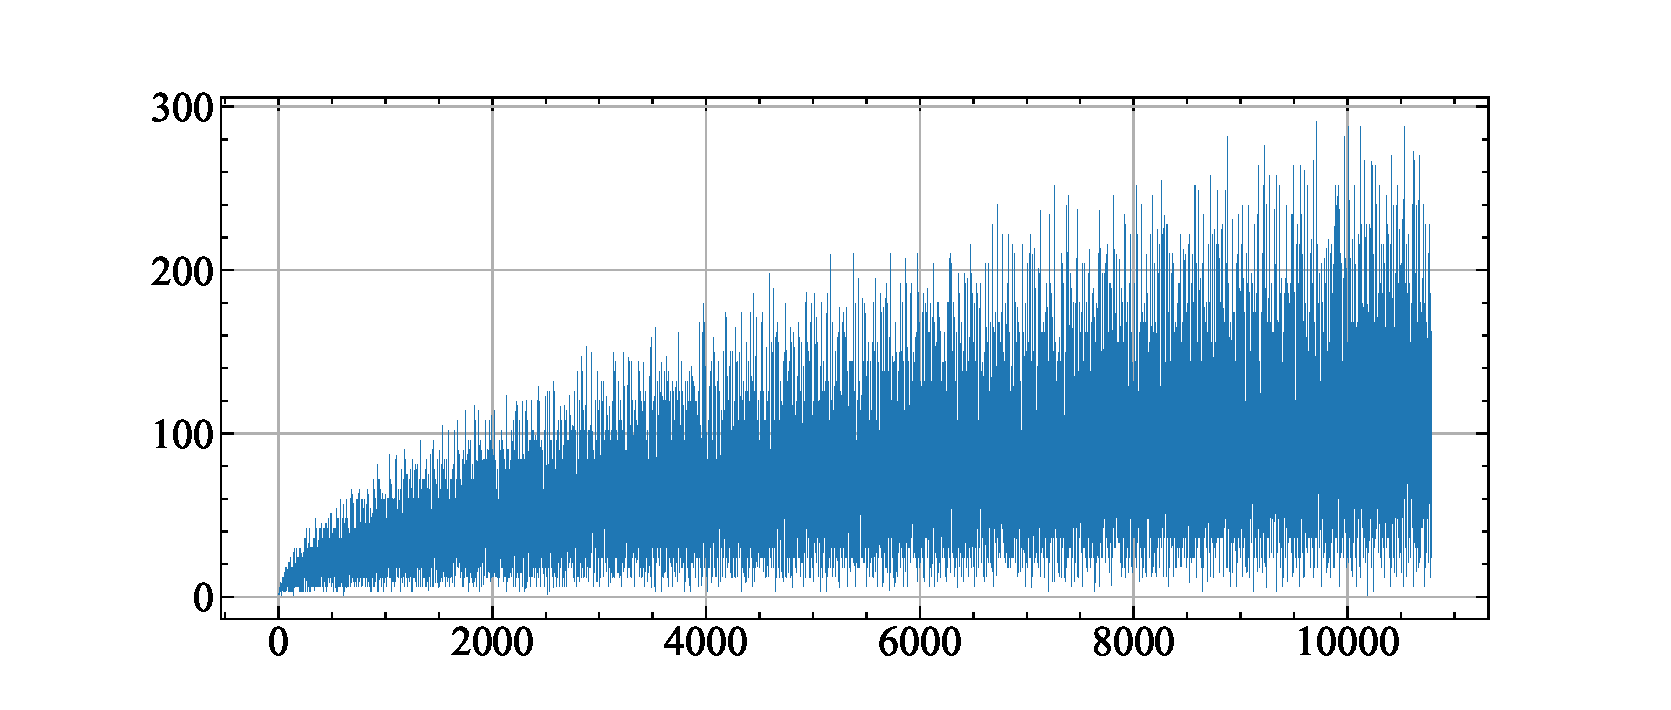
\includegraphics[width=\textwidth]{../../Figure/热统/系综理论/三维盒子自由粒子简并度.eps}
    \caption{三维盒子中自由粒子的能级简并度示意图。横轴表示能级编号，也就是0表示基态，1表示第一激发态，以此类推。纵轴是相应能级的简并度。从图中大致可以看出，能级简并度随能量的变化类似抛物线，后面我们将采用近似手段，显式的给出这一关系}
    \label{fig:box-degeneracy}
    \end{figure}
    \item 角动量量子化。原子物理中提到，粒子的角动量，包括轨道角动量和自旋角动量，都是量子化的，既包括大小的量子化也包括取向的量子化，前者由量子数\(j=0,1,2,\dots\)表示，后者由量子数\(m_j(\abs{m_j}=0,1,\dots,l)\)表示。
    \begin{enumerate}
        \item 轨道角动量量子化——转动能级。考虑一个转动惯量为\(I\)的分子，它的转动动能可以表示为\(E_l=\frac{L^2}{2I}=\frac{l(l+1)\hbar}{2I}\)。类似氢原子核外电子，对于某个确定的能级即\(l\)固定时，\(m_l\)有\(2l+1\)个值，每个值对应一个不同的定态，它们的能量都是\(\frac{l(l+1)\hbar}{2I}\)，因此转动能级的简并度是\(2l+1\)
        \item 自旋角动量量子化——磁能级。我们考虑一个自旋为\(\frac{1}{2}\)的粒子，粒子的自旋会产生一个磁矩，在沿\(z\)轴的匀强磁场中，该磁矩会产生两个磁能级\footnote{其实就是原子物理中学习的塞曼效应，此处仅考虑自旋。帮读者进行简单的回忆：一个磁矩\(\mathbf{\mu}\)在磁场\(\mathbf{B}\)中的能量为\(E=-\mathbf{\mu}\cdot\mathbf{B}=-\mu_zB\)。对\(\frac{1}{2}\)自旋，朗德\(g\)因子为2，所以有\(\displaystyle\mu_z=2\frac{q}{2m}m_s\hbar=\pm\frac{q\hbar}{2m}\)}：\(E_{-}=-\frac{q\hbar}{2m}B,E_{+}=\frac{q\hbar}{2m}B\)分别对应\(m_s=\frac{1}{2}\)和\(m_s=-\frac{1}{2}\)。我们记\(\frac{q\hbar}{2m}=\mu_B\)，则磁能级可以表示为\(E_{\pm}=\pm\mu_B B\)。注意这里的\(\mu_B\)并不是玻尔磁子，\(q\)表示粒子的电荷，可正可负，\(m\)表示粒子的质量。因此，\(E_{\pm}\)两个能级的大小取决于粒子的电性即\(q\)的正负。这两个磁能级都是非简并的。倘若粒子的能级是两个非简并能级，由这样的粒子组成的系统，称为二能级系统，是统计力学教学中常用的toy model
    \end{enumerate}
\end{enumerate}
\begin{example}
    求解无限深势阱中的自由粒子的能级。
    \begin{solution}
    所谓的无限深势阱就是盒子，我们从一维无限深势阱谈起，推广只三维无限深势阱。

    在一维无限深势阱中，设势能在\([0,L]\)之间为0。粒子的能级和定态波函数由定态薛定谔方程给出，即
    \begin{equation*}
        \dv[2]{\psi}{x}+\frac{2mE}{\hbar^2}\psi=0\quad (E>0)
    \end{equation*}
    其中\(\psi\)为定态波函数，\(E\)就是能级\footnote{自由粒子，能量仅为动能一定为正}。对于这样一个二阶微分方程，我们需要两个初值条件，但物理上给不出来，此外这个方程本质是数理方法中学习的本征方程，不需要初始条件而需要边界条件。我们直接给出两个边界条件\footnote{不用细究这两个边界条件的由来，量子力学中先求解一维对称深势阱的定态波函数，接着令势阱高度趋于无穷，可得波函数在势阱边界处的值趋于0}
    \begin{equation*}
        \psi(0)=\psi(L)=0
    \end{equation*}
    因为定态薛定谔方程中有一个未知参数\(E\)，即使利用两个边界条件我们也无法完全确定\(\psi\)，在数理方法课程中，即本征方程的解有一个无所谓的系数因子，因为本征解要和非本征解相乘才是偏微分方程的解。但在这里，定态波函数是特殊的波函数，是有物理实在意义的，我们引入波函数的概率归一化条件
    \begin{equation*}
        \int_{0}^{L}\abs{\psi}^2\dd x=1
    \end{equation*}
    所有条件准备就绪，我们正式求解。这个方程的形式大家很熟悉，间谐振动方程的解为 
    \begin{equation*}
        \psi(x)=A\sin(kx)+B\cos(kx)\quad k=\sqrt{\frac{2mE}{\hbar^2}}
    \end{equation*}
    代入边界条件有
    \begin{equation*}
        \psi(0)=B=0\quad \psi(L)=A\sin(kL)+B\cos(kL)=0
    \end{equation*}
    \(B\)已经是0了，那么\(A\)就一定不是0，不然解就没有意义了，所以我们有
    \begin{equation*}
        \sin(kL)=0\Rightarrow k=\frac{n\pi}{L}\quad (n=1,2,3,\dots)
    \end{equation*}
    到这里我们就得到了能量量子化即能级公式
    \begin{equation*}
        E_n=\frac{\hbar^2k^2}{2m}=\frac{n^2\hbar^2\pi^2}{2mL^2}\quad (n=1,2,3,\dots)
    \end{equation*}
    为了完全确定波函数，我们利用概率归一化条件
    \begin{equation*}
        \int_{0}^{L}\abs{A}^2\sin[2](kx)\dd x=1
    \end{equation*}
    我们规定A为正实数，则\(A=\sqrt{\frac{2}{L}}\)，定态波函数为
    \begin{equation*}
        \psi_n(x)=\sqrt{\frac{2}{L}}\sin\left(\frac{n\pi x}{L}\right)
    \end{equation*}
    反复出现的\(n\)就是量子数，一个确定的\(n\)，对应一个唯一的定态波函数即量子态，不难发现一个能级对应唯一一个\(n\)，也就是一维无限深势阱中的自由粒子能级是非简并的。

    上述求解过程非常简单，数理方法中学习的弦振动本征方程也是这样的步骤。不过要强调一点我们现在求解的是一个粒子的定态，而不是一堆质点在振动。数学上，这一差别表现在公式\(k=\sqrt{\frac{2mE}{\hbar^2}}\)。弦振动方程分离变量时，\(k^2\)本身就是本征值\footnote{也有不少教科书用\(\lambda\)表示弦振动方程分离出的本征值，但我们知道分离出的这一本征值的平方根，其物理意义是波的空间振动频率，因此这里直接用\(k^2\)表示，用\(k\)表示波的空间频率也算是物理的约定俗成了}，而薛定谔方程分离变量得到定态薛定谔方程时，\(E\)才是本征值，不过数学知识告诉我们\(\sqrt{\frac{2mE}{\hbar^2}}\)表示的是定态波函数的空间频率，也就是\(k=\sqrt{\frac{2mE}{\hbar^2}}\)这个公式左边表征波而右边表征一个粒子，这正是波粒二象性的体现。把这个公式和非相对论自由粒子的能动量关系\(p=\sqrt{2mE}\)放在一起，我们立即可以得到\(k=\frac{p}{\hbar}\)，这正是德布罗意关系式。我们的讨论出发点是非相对论自由粒子，但其实德布罗意关系式是恒成立\footnote{打个趣：\(k=\sqrt{\frac{2mE}{\hbar^2}}\)和\(p=\sqrt{2mE}\)都只在非相对论自由粒子时成立，负负得正得到了一个恒成立的\(k=\frac{p}{\hbar}\)}的，因为它来自于动量算符的本征矢，大家会在量子力学中详细学习。正因为它恒成立，后文涉及到极端相对论粒子的统计时，我们会再次使用德布罗意关系式。

    接下来讨论二维无限深势阱，我们不可能也没必要再次从头细致推导，类似于二维波动方程，我们对分离变量得到的空间方程再次分离变量得到两个本征方程，分别求解即可。二维的定态薛定谔方程如下
    \begin{equation*}
        \pdv[2]{\psi}{x}+\pdv[2]{\psi}{y}+\frac{2mE}{\hbar^2}\psi=0\quad (E>0)
    \end{equation*}
    设\(\psi(x,y)=\psi_x(x)\psi_y(y)\)，记\(k^2=\frac{2mE}{\hbar^2}\)，一番倒腾之后可以得到
    \begin{equation*}
        \frac{1}{\psi_x}\dv[2]{\psi_x}{x}=-\frac{1}{\psi_y}\dv[2]{\psi_y}{y}-k^2=-k_x^2
    \end{equation*}
    其中\(k_x^2\)是第一个本征值，由此我们得到了两个本征方程
    \begin{equation*}
        \begin{cases}
            \displaystyle \dv[2]{\psi_x}{x}+k_x^2\psi_x=0 \\
            \displaystyle \dv[2]{\psi_y}{y}+k_y^2\psi_y=0\quad k_y^2=k^2-k_x^2
        \end{cases}
    \end{equation*}
    \(k_y^2\)就是第二个本征值。对于这两个本征方程的求解不再赘述，我们直接给出最终的能级公式和定态波函数
    \begin{equation*}
        \begin{cases}
            \displaystyle E_{n_x,n_y}=\frac{\hbar^2k^2}{2m}=\frac{\hbar^2\pi^2(n_x^2+n_y^2)}{2mL^2} \quad (n_x,n_y=1,2,3,\dots) \\
            \displaystyle \psi_{n_x,n_y}(x,y)=\frac{2}{L}\sin\left(\frac{n_x\pi x}{L}\right)\sin\left(\frac{n_y\pi y}{L}\right)
        \end{cases}
    \end{equation*}
    可以看到，从二维开始，粒子的能级就开始简并了，值得一提的是这里能级发生简并不是偶然的，大家在量子力学中会深入学习。至于三维无穷深势阱中的自由粒子，求解过陈无非只是多了一个维度，我们直接给出结果
    \begin{equation*}
        \begin{cases}
            \displaystyle E_{n_x,n_y,n_z}=\frac{\hbar^2k^2}{2m}=\frac{\hbar^2\pi^2(n_x^2+n_y^2+n_z^2)}{2mL^2} \quad (n_x,n_y,n_z=1,2,3,\dots) \\
            \displaystyle \psi_{n_x,n_y,n_z}(x,y,z)=\left(\frac{2}{L}\right)^{\frac{3}{2}}\sin\left(\frac{n_x\pi x}{L}\right)\sin\left(\frac{n_y\pi y}{L}\right)\sin\left(\frac{n_z\pi z}{L}\right)
        \end{cases}
    \end{equation*}
    至此我们求出了无限深势阱中的自由粒子能级，倘若有读者感到头疼，不必苦恼，这是热统课程中唯一定量计算的量子力学内容，后续再也没有了。读者可能发现了我们的求解默认了无限深势阱是方的，也就是默认盒子是立方的，但实际上比如一个气体系统，约束它的盒子可以是长方体甚至是乱七八糟不规则的容器，我们基于立方体内自由粒子的统计规律能用在任意形状容器吗，答案是可以的\footnote{扔一句话在这里是极不礼貌的，但我也不知道为什么可以，也没有教材讨论这一点，大家都从立方盒子开始统计。分享跟大家一句打趣的话：我们的模型已经这么粗糙了，为什么不让它更粗糙一点呢？}。
    \end{solution}
\end{example}

我们讨论了一些简单情形下粒子的能级，但统计力学关注的是大量粒子构成的系统。对于系统，不难想到它的定态\footnote{一个系统有量子态，系统一般由大量同种粒子构成，单个粒子也有量子态，两者显然不同，但本笔记不会可以区分，请读者联系上下文自行判断}也是量子化的。倘若粒子之间无相互作用，那么系统的能量就是各粒子能量和，单个粒子的能级一般比较易得，系统的定态能量和定态是比较好计算的。但如果粒子间有相互作用，系统的能量就包括相互作用能，那么系统的能量量子化会很复杂，对这种系统的统计仍在系综统计的框架下，不过人们发展了许多特殊方法，在本科热统课程，基本不会涉及，本笔记也没有涉及。因此我们后文的所有讨论都建立在系统内粒子无相互作用的假设上。关于这点后文会再次说明。

对于无相互作用系统，系统的能量是各粒子能量之和，那么如何确定系统的不同量子态呢？这就引出了量子力学第二个显著不同于经典力学的地方：全同粒子不可分辨。

\subsection{全同粒子不可分辨}

全同粒子，就是质量、电荷、自旋等内禀属性相同的粒子，比如氢原子中的电子和钠原子中的电子就是全同粒子，不同原子核发生\(\alpha\)衰变放出的\(\alpha\)粒子也是全同粒子。显然，全同粒子是一个客体概念，跟动力学无关，经典力学也有全同粒子。

既然全同粒子的内禀属性完全相同，那么我们如何区分一堆全同粒子呢？经典力学视角下，我们可以利用轨迹区分，全同粒子的内禀属性相同，但位置总是不一样的，在整个运动过程中，全同粒子的轨迹总是不一样的，所以我们可以用轨迹辨认不同的全同粒子。比如两个相向运动的完全相同的刚体小球，碰撞后两者会背离运动，我们能追踪整个轨迹进而区分这两个完全相同的刚体小球。

在量子力学的视角下，事情就没有这么美妙了。量子力学中没有轨迹的概念，一个粒子的状态由波函数描述，波函数的模方表示粒子在空间中各处出现的概率。假如在我们考查的区域里，两个全同粒子的波函数相互交叠，那么我们测量两个粒子的位置，会在两个地方随机的发现两个粒子，除此之外我们什么也不知道了，所以我们无法区分这两个全同粒子，我们所知道的仅仅是有两个粒子而已。

但这说实话是有点匪夷所思的，比如读者体内的一个电子和月球上的岩土中的一个电子，这显然是全同粒子，但要说它们两个不可区分太瞎扯了，很明显一个在地球\footnote{应该没有读者不在地球吧}一个在月球。没错，这两个全同粒子是可以区分的，也就是量子力学中全同粒子不可分辨是有前提的，正如上一段所说，两个全同粒子的波函数必须交叠。倘若两个全同粒子的波函数互不重叠，也就是一个粒子随机出现的所有可能位置，另一个粒子都不可能出现，那么虽然两个粒子还是没有轨迹，但总体上我们可以划定两个空间范围进而区分它们。正因为量子力学中全同粒子是否可以区分，依赖于粒子的波函数，我们可能会遇到两个全同粒子初始时刻波函数不交叠进而可以区分，一段时间后波函数交叠又变得不可区分这种神奇现象。

具体到我们的统计物理课程，我们的统计以量子力学为基础，此处列举两个例子。对于晶体中的原子，我们知道晶体是由原子有序排列而构成的，晶体中的某个原子不可能随机出现在晶体中的任何位置，只会在晶格附近局域范围内运动，因此晶体中的原子是可以区分的。在量子力学中，我们要区分全同粒子，必须要求粒子只在一个小范围内运动，因此对于可区分全同粒子构成的宏观系统，我们称之为定域系统。对于一个盒子内的气体分子，每个气体分子的波函数都弥散在整个盒子里，没有任何东西阻止气体分子在盒内的运动，因此这些气体分子是不可区分的。全同粒子不可分辨是量子力学出现后诞生的概念，但吉布斯为了解决了吉布斯佯谬，指出了盒子中的气体分子必须不可分辨，这是超越时代的见解。

关于全同粒子不可分辨的特殊之处还没有结束，人们发现，对于不可分辨的全同粒子，可以分为两类，它们的统计性质截然不同。在阐述这两类差别之前，我希望读者能建立一种观念：全同粒子不可分辨，但量子态可以分辨，因此我们区分不同量子态上的全同粒子数目，而不是区分全同粒子的量子态。这一观点对于理解后续的量子统计是必须的，对读者日后的量子力学学习也是有裨益的。

人们发现，有一种全同粒子，我们称之为玻色子，可以多个粒子占据同一量子态；另一种全同粒子，我们称之为费米子，不能两个及以上粒子占据同一量子态。也就说：对于玻色子构成的系统，一个量子态上，可以有任意多的玻色子；对于费米子构成的系统，一个量子态上至多有一个费米子，要么没有费米子，有的话只能有一个。那么我们如何知道一个粒子是玻色子还是费米子呢？大自然很神奇的留下了一条规律即自旋—统计定理：自旋为整数\footnote{一个粒子的自旋只能是\(0,1,2,\dots\)或\(\frac{1}{2},\frac{3}{2},\frac{5}{2},\dots\)，前者称为整数，后者称为半整数。比如电子自旋为\(\frac{1}{2}\)就是半整数，\(\alpha\)粒子自旋为0，是整数}的粒子是玻色子；自旋为半整数的粒子为费米子。对于费米子的这种性质，大家在高中应该就有所接触，即泡利不相容原理，电子是费米子，自然遵循泡利不相容原理。此外，玻色子的复合仍然是玻色子，偶数个费米子的复合是玻色子，奇数个费米子的复合仍是费米子。比如\(\alpha\)粒子是两个质子两个中子，质子和中子都是费米子，因此\(\alpha\)粒子就是玻色子。

回到上一小节结尾提出的问题，全同粒子构成的系统，如何确定系统的量子态？实际上这个问题对于统计物理来说，是过于严苛的，我们马上就会看到，统计物理只在意系统的量子态个数，而并不关心量子态的具体表达式。因此这个问题没有答案，下面我举个例子，大家体会一下。

\begin{example}
    考虑由100个无相互作用的粒子构成的二能级系统，系统的总能量是0。这个系统有多少个可能的量子态呢？
    \begin{solution}
        倘若100个粒子是可以区分的，那么每个粒子的量子态都确定了，系统的量子态自然就确定了\footnote{对这句话陌生的读者，我们可以把它翻译成经典版本：确定质点系每个质点的状态（即位矢和速度），我们就确定了质点系的状态}。所以系统量子态的个数就是这100个粒子可能的量子态组合的个数。假如不考虑任何限制，纯粹的数学组合，这个系统可能有\(2^{100}\)个量子态，但实际上系统是有限制的，系统能量为0，因此我们要在100个粒子中选择50个粒子，令它们位于基态，剩下50个粒子处于第一激发态，显然这样的选择有\(C_{100}^{50}\)个。也就是系统有\(C_{100}^{50}\approx\exp(66.784)\)个可能的量子态。这是一个极大的数字，而我们现在仅仅考虑了100个粒子。而且我们也看到了，对单个粒子来说能级是不简并的，但对于系统，能级是大量简并的，对于系统能量为0这个能级，简并量子态数目达到\(\exp(66.784)\)。

        倘若100个粒子是不可分辨的，我们还要指定粒子是玻色子还是费米子。如果粒子是费米子，根据泡利不相容原理，粒子只有两个量子态，因此系统最多两个费米子，显然不可能，所以100个粒子是玻色子。对于不可分辨的粒子，我们要区分不同量子态有几个粒子\footnote{如果执意从粒子出发进行计算，对这个简单系统是可行的：同样，我们选择50个粒子位于基态，但这100个粒子完全相同，因此挑选50个粒子只有1种选法}，也就是说确定了各量子态的粒子数目，就确定了系统的量子态。如果还是不考虑任何限制，纯粹的数学组合，系统可能有101个量子态。考虑到系统能量为0，那么基态有50个粒子，第一激发态有50个粒子，系统只有1个可能的量子态。可以看到，考虑到全同粒子不可分辨性后，系统可能的量子态数目大大减少。
    \end{solution}
\end{example}


\section{系综统计基本原理}
\subsection{系综的观念}
从本节开始，我们正式学习统计物理或者更准确的说是系综统计的内容。首先介绍一个反复出现但一直未解释的概念，系综。系综之于现代统计物理好比集合之于现代数学，系综是所有理论推导的基础概念。为了清晰的表述这个概念，必须要同时介绍现代统计物理所遵循的统计观念。

统计力学试图从微观规律出发推导宏观系统的各种热力学量，为了达成这一目的，我们必须找到各热力学量的微观对应。更进一步，根据热力学的知识，我们不需要\footnote{实际上也不可能，很多热力学量本身就是针对宏观系统定义的，无论针对单个微观粒子或者微观状态确定的系统，它们都没有意义}统计出所有的热力学量，实际上在后续的学习中，我们主要统计系统的内能和熵，别的热力学量都通过热力学关系推导。关于熵的统计我们按下不表，关于内能的统计，热学课程中学过，内能就是各粒子能量的和，这就是分子动力学视角的统计力学，在序章我们已经提及，这种视角发展在统计物理初期，难以处理粒子之间的相互作用，后续被系综统计取代。

那么系综到底是什么呢？系综统计如何计算内能呢？对于一个平衡态系统，其往往是满足一定约束\footnote{我们考虑的所有系统体积都恒定不变，对于实际上体积会变得系统，我们后文会说明怎么处理}的，比如孤立系统它的\(\left(N,V,E\right)\)是确定的，与热源接触的封闭系统其\(\left(N,V,T\right)\)是确定的，与热源和粒子源同时接触的开放系统其\(\left(\mu,V,T\right)\)是确定的。此外系统是平衡态表明它的所有热力学量均不变，但这个不变和上述的约束有本质的区别。不同系统满足的不同约束是事先给定的，是我们理论计算的出发点，而其余热力学量不变是实验观测到的，是我们理论计算的终点。也就是我们的理论要计算出一个唯一的热力学量，而计算过程中它可以是不唯一的。由此就引出了系综的概念。

对于一个满足某种约束的系统，显而易见，这个系统可以是不同的微观状态，允许的微观状态数往往还是巨大的。所谓的微观状态，就是上一节反复提及的系统量子态\footnote{在本笔记中，我们用\(s\)表示系统不同的量子态，不是不同的能级！！！它表示一个抽象的状态，在实际操作时我们要把它变成具体的量子数}。针对这样的一个实际系统，我们假想一系列存在于我们思维里的虚拟系统，即真实系统的“思维副本”，这些系统的特点是与真实系统满足同样的约束，但它们的微观状态是确定的，而且要遍及系统允许的所有微观状态。更准确地说，假设我们虚拟构造了\(\tilde{N}\)个系统\footnote{\(\tilde{N}\)是趋于无穷的，这样才能利用大数定律保证频率收敛于概率，这是完全可行的，因为这些系统都是思维副本，想制造几个就制造几个}，这些系统中处在\(s\)这个量子态的系统有\(\tilde{n}_s=P_s\tilde{N}\)个。其中\(P_s\)是系统\(s\)这个量子态出现的概率\footnote{读者在学习热统课程时大多正在或者已经学习了量子力学，我们已经接触了三种概率，一种是经典力学中的概率，比如抛硬币正反面朝上；一种是系宗理论中量子态的概率；一种是量子力学测量结果的概率。三种概率的数学意义都是一致的，物理意义上它们有什么区别和联系？这个问题是笔者瞎想的，各位读者权且一听，欢迎交流}，计算这个概率是统计物理的核心任务。对于这样虚拟出来的一堆系统，构成的集合就是系综。

系综中的一堆系统满足同一个约束，但微观状态不一定相同，由此各系统的能量\(E\)也就不一定相同。系综统计认为真实系统的内能，是系综中所有系统的能量的均值，根据大数定律，这意味着系统的内能，是系统微观状态能量的期望，即
\begin{equation}
    U=\expval{E}=\sum_s E_sP_s
\end{equation}
这种统计视角就是系综统计，\(E_s\)表示系统的能量，而这个能量的期望就是系统的内能。格外强调，这里的能量是系统的能量，是一个宏观大小的量，而不是某个微观粒子的能量。系统能量本身就包含粒子之间的相互作用，所以系综统计可以自然地处理相互作用系统。这里的微观状态指的是系统本身的微观状态，而不是某个粒子的状态。再次强调，系综统计是对系统本身的统计。这种统计观点，在部分教科书里以“热力学量的时间平均等于系综平均”来表述，因为我们针对系统热力学量的测量总是在一个有限时间内的持续测量，测量结果是这个时间内的平均值。

一个值得考虑的问题是：这种系综统计的视角真的成立吗？也就是为什么系统的内能等于系统能量的期望，乍一看这貌似很合理的，但它确实没有更底层的规律支撑了，是一个纯粹的统计规律，我们要假定它成立，它的正确性是由系综统计的推论与实验相符来保证的。另一方面来看，系综统计完全回避了一个力学问题，就是平衡态系统，其微观状态的演化问题，这是一个动力学的问题，而系综统计仅涉及到系统的定态，这是一个纯粹的静态问题。关于系综统计更深层的研究，特别是统计规律和动力学的关联，大家凭兴趣自行了解，从教学的角度来说，这是我们理论的出发点。

最后多提一嘴，系综这个概念在物理学史上提出来时肯定不是上述表述，因为那个时候量子力学还在睡觉。正如我们在本章开头所论述的，倘若跟随经典的系综定义进入统计物理，我们的统计必然是建立在经典力学基础上的，还需要另外打上量子力学的补丁，因此本笔记没有采用这种讲法。但希望读者也去学习一下这部分基于经典的内容，能加深对统计物理统计基础的理解。

\subsection{等概率原理与玻尔兹曼熵}

所有的系统中，孤立系统是最基础的，因为我们总是可以扩大我们的研究对象使之成为一个孤立系统，所以我们要先研究孤立系统的统计。而正是因为孤立系统太基础了，我们要提出两个公理化的假定，来完成针对孤立系统的统计。

首先，给定一个孤立系统，因为系统与外界是完全隔绝的，所以系统的\(\left(N,V,E\right)\)是固定不变的，对于这样一个系统的各微观状态，我们提出等概率原理：平衡态孤立系统所有可能的微观状态出现的概率相等。记孤立系统所有可能的微观状态数为\(\Omega(N,V,E)\)，则等概率原理的数学描述就是
\begin{equation}
    P_s=\frac{1}{\Omega}
\end{equation}
其次，我们定义孤立系统的熵，由玻尔兹曼公式给定，即
\begin{equation}
    S=k\ln \Omega
\end{equation}
这里的\(k\)就是玻尔兹曼常数\footnote{物理中常用\(k\)表示某个比例系数，为了避免混淆玻尔兹曼常数用\(k_B\)表示，但在统计物理课程中，玻尔兹曼常数频繁出现，因此我们仍用\(k\)表示以简化书写}，作为比例系数被引入玻尔兹曼公式，后续我们用这套理论处理理想气体的统计，能确定玻尔兹曼常数在国际单位制下的值。

由孤立系统构成的系综称为微正则系综。等概率原理告诉我们，微正则系综中的不同系统，它们出现的概率相同。这是第一性的，我们把等概率原理作为系综统计的公理，它是一个纯概率的假设，它的正确性是由被实验不断证实的统计物理理论而保证的。如何从动力学出发推导等概率原理依然是统计物理的基础问题，从教学的角度出发，它就是无需证明的公理。

对微正则系综，等概率原理貌似没有任何作用，因为孤立系统的能量为定值，所以计算内能时我们无须在意各微观状态的概率分布，即
\begin{equation}
    U=\sum_s E_sP_s=E\sum_s P_s =E
\end{equation}
后续在其他系综理论中，我们将体会到等概率原理的作用。

相比于等概率原理，玻尔兹曼公式对微正则系综就显得十分重要了，因为它直接给出了孤立系统的熵。给定孤立系统的\(\left(N,V,E\right)\)，借助量子力学求出系统可能的微观状态数\(\Omega(N,V,E)\)，我们就直接得到了系统的熵。希望读者能明确，玻尔兹曼提出玻尔兹曼熵肯定不是无稽之谈，背后有一定的理论基础和逻辑推演\footnote{感兴趣的同学可以自行查找资料，关于统计物理各种概念的发展不可谓不曲折，可以说是基础物理理论最坎坷的了}，但这不能取代玻尔兹曼公式的公理性，它作为一个公理给出了孤立系统的熵，它同样没有更基础的严格证明。我们在提出等概率原理的时候强调了平衡态，但提及玻尔兹曼熵只强调了孤立系统，这里有一个微妙的适用条件。仅从玻尔兹曼熵的表达式\(S=k\ln \Omega(N,V,E)\)来说，给定系统的三个约束，原则上我们一定能计算出一个熵，这跟系统本身是否平衡没有关系。因此玻尔兹曼熵可以推广到非平衡孤立系统，不过此时计算出的熵没有各种热力学性质；对于平衡态孤立系统，玻尔兹曼熵与热力学中的克劳修斯熵是等价的，可以参与各种热力学的理论计算。

玻尔兹曼熵赋予了宏观熵微观意义。孤立系统的微观状态数越大，我们对系统的认识就越少，因为对于孤立系统我们只知道其\((N,V,U)\)三个宏观量，这种对系统认知的缺失，也可以理解为系统的混乱程度，因此玻尔兹曼熵一个重要的物理意义就是表明了熵是孤立系统混乱程度的度量。但是玻尔兹曼熵只能用在孤立系统，对于非孤立系统，我们如何在保证熵表征系统不可知程度的同时给出熵新的公式，后文我们会提到吉布斯熵，回答这一问题。

在本小节的最后，我们要再次强调，等概率原理和玻尔兹曼熵公式是针对孤立系统的两条基本假设，它们构成了系综统计整个体系的基础，后续所有的系综理论都可以由这两个基本假设推出。它们在系综统计中的地位，类似狭义相对性原理和光速不变原理在狭义相对论时空观中的地位，它们的正确性是由整个系综理论保证的。

\subsection{宏观系统的最概然特性}

为了得到系统的熵，我们要计算系统的微观状态数，这当然是一个技术性问题，不应该出现在本节。不过对于我们研究的宏观系统，也就是\(N\)极大的系统，宏观系统的微观状态数满足一个特性，这个特性是如此地重要以至于没有这个特性我们要修改统计物理的基本假设。为了说明这一特性，我们从一个具体的例子入手考虑。

我们举例的对象依然是二能级系统，这是一个足够简单又能说明许多问题的模型。我们的计算将涉及很多阶乘运算，这里要引入一个计算阶乘的近似公式——斯特林公式，它在统计物理中被广泛使用。
\begin{equation}
    \ln N! \approx N\ln N-N+\frac{1}{2}\ln(2\pi N)\approx N\ln N-N
\end{equation}
把上述公式变成指数形式，就得到了阶乘的近似式。上述公式第一步近似的精度极高，在\(N\)不怎么大的时候就可以使用。统计物理中\(N\)表示系统的粒子数，一般是极大的，因此可以把\(\frac{1}{2}\ln(2\pi N)\)当成小量略去，得到稍粗糙的斯特林公式。在本小节，我们要细致地说明宏观系统的特性，因此使用第一步近似，后文实际计算宏观系统的热力学量时主要使用第二步近似。

假设二能级系统由\(N\)个可分辨且无相互作用的粒子，粒子的能级为\(-\varepsilon\)和\(\varepsilon\)，系统总能量为\(E=0\)。这样一个系统的微观状态数我们已经计算过为\(\Omega_{\text{total}}=C_{N}^{\frac{N}{2}}\)。下面我们用另一个方法计算系统的微观状态数。

我们假想把整个系统按粒子数一分为二，得到两个子孤立系统对\(A\)和\(B\)，两个子系统的粒子数均为\(\frac{N}{2}\)，因为两个子系统的能量和为0，因此确定了\(A\)系统的能量，\(B\)系统能量就随之而定了。对于子系统\(A\)，它是一个粒子数为\(\frac{N}{2}\)的二能级系统，显然它的能量由基态的粒子数目决定，不妨设其为\(N_1\)。一旦我们确定\(N_1\)，\(A\)系统的能量就确定了，接着\(B\)系统的能量随之而定，因此我们能确定这两个子系统的微观状态数，两者相乘就是此时系统的微观状态数，那么系统的总微观状态数显然是上述微观状态数对\(N_1\)求和，即\begin{equation*}
    \Omega_{\text{total}}=\sum_{N_1}\Omega_{A}(N_1)*\Omega_{B}(N_1)
\end{equation*}
其中\(\Omega_{A}(N_1)\)显然为\(C_{\frac{N}{2}}^{N_1}\),根据对称性不难得到\footnote{感觉难得到的同学可以把\(B\)系统的基态粒子数目用\(N_1\)表示出来}\(\Omega_{B}(N_1)\)也为\(C_{\frac{N}{2}}^{N_1}\)。因为\(B\)系统的“兜底”作用，\(A\)系统的能量没有限制，也就是\(N_1\)可以取遍\(0\)到\(\frac{N}{2}\)，综上我们有
\begin{equation*}
    \Omega_{\text{total}}=\sum_{N_1=0}^{\frac{N}{2}}\left(C_{\frac{N}{2}}^{N_1}\right)^2
\end{equation*}
这种计算方法可以认为是化整为零，我们所做的事实际上是把系统的总能量分配给两个子系统，对于每种分配方式，我们计算出一个系统的微观状态数，对所有的分配方式求和，就得到了系统总的微观状态数。对于二能级系统这属实是多此一举，我们举着个例子是为了说明宏观系统的特性。这个求和式本身是有解析的计算方法的，结果也确实是\(C_{N}^{\frac{N}{2}}\)。但这是因为二能级系统过于简单了，而且我们的任务也不是严格地把这个求和计算出来。

这种计算思路意味着，每一个\(N_1\),对应着一种能量分配，进而对应一个系统的微观状态数。对于使系统微观状态数取最大值的分配，我们称为最概然分配，此时的微观状态数称为最概然微观状态数，不妨记为\(\Omega^*\)。观察求和项\(\left(C_{\frac{N}{2}}^{N_1}\right)^2\)，不难得到求和项的最大值为\(\left(C_{\frac{N}{2}}^{\frac{N}{4}}\right)^2\)，此时\(N_1=\frac{N}{4}\)。也就是说最概然分配是\(N_1=\frac{N}{4}\)，最概然微观状态数\(\Omega^*=\left(C_{\frac{N}{2}}^{\frac{N}{4}}\right)^2\)。接下来我们尝试是否可以用\(\Omega^*\)来近似\(\Omega_{\text{total}}\)，也就是用求和项的最大值来代替整个求和。

为此我们要计算两者的比值，令
\begin{equation*}
    \eta=\frac{\Omega^*}{\Omega_{\text{total}}}=\frac{\left[\left(\frac{N}{2}\right)!\right]^4}{N!\left[\left(\frac{N}{4}\right)!\right]^4}
\end{equation*}
我们可以直接使用斯特林公式开始计算，但笔者更喜欢取对数，利用对数形式的斯特林公式，因此我们取对数
\begin{equation*}
    \begin{split}
        \ln \eta&=4\ln \frac{N}{2}!-\ln N!-4\ln \frac{N}{4}! \\
        &\approx 4\left(\frac{N}{2}\ln \frac{N}{2}-\frac{N}{2}+\frac{1}{2}\ln 2\pi\frac{N}{2}\right)-N\ln N+N-\frac{1}{2}\ln 2\pi N-4\left(\frac{N}{4}\ln \frac{N}{4}-\frac{N}{4}+\frac{1}{2}\ln 2\pi\frac{N}{4}\right) \\
        &=2\ln \pi N-\frac{1}{2}\ln 2\pi N-2\ln \frac{\pi}{2}N \\
        &=-\frac{1}{2}\ln \pi N+\frac{3}{2}\ln 2
    \end{split}
\end{equation*}
最后的\(\frac{3}{2}\ln 2\)可以直接略去，即\(\eta\approx \frac{1}{\sqrt{\pi N}}\)。对于宏观系统，\(N\)是很大的，因此在理论分析的时候我们可以直接令\(N\to \infty\)，这被称为热力学极限。在热力学极限下，\(\eta\to 0\)，这表明最概然微观状态数在总微观状态数里是个小量，可以略去不计的，我们用它来近似总微观状态数显然是不可能的。但事实真是如此吗？对于统计物理，真正有热力学意义的熵，是微观状态数的对数，而不是微观状态数本身，因此我们进一步比较一下用最概然微观状态数计算的近似熵和真实熵的比值\footnote{读者可以用粗糙的斯特林公式计算一下这个比值，看看结果有何特殊之处}，即
\begin{equation*}
    \frac{S^*}{S}=\frac{\ln \Omega^*}{\ln \Omega}=\frac{2\ln \frac{N}{2}!-4\ln \frac{N}{4}!}{\ln N!-2\ln \frac{N}{2}!}\approx \frac{N\ln2-\ln\pi N+2\ln2}{N\ln2-\frac{1}{2}\ln\pi N+\frac{1}{2}\ln2}
\end{equation*}
热力学极限下，显然有\(\frac{S^*}{S}\to 1\)即最概然微观状态数计算出的近似熵和实际的熵是等量级的，完全可以近似。这不可谓不神奇，简直像自然界事先预备好了，对于不可近似的微观状态数，取对数得到的熵却是可以近似的，而恰好只有熵才是有意义的。

从数学上来说，这得益于对数的“压缩”特点。指数函数增长极快，因此能放大自变量的微小变化，而对数函数作为指数函数的反函数，能极大缩小自变量的变化。更具体来说，只要两个无穷大的比值不是指数发散的，分别取对数后，对数的比值就是收敛的。不难举出这样的例子，比如\(x^2\)与\(\mathrm{e}^x\)作商，是指数发散\footnote{当然这里是指数收敛，取倒数就是指数发散，因此称为指数发散没有问题}的，对数的比值为\(\frac{2\ln x}{x}\)依然是发散的；而\(x^2\)与\(x^3\)作商是多项式发散的，因此对数比值\(\frac{2\ln x}{3\ln x}\)是收敛的。最概然微观状态数相较于总微观状态数就是多项式差距即\(\frac{\Omega^*}{\Omega_{\text{total}}}\propto N^{-1/2}\)，因此对数的比值就是收敛的。

经过对两个比值的分析，我们得到可以用最概然分配的熵\footnote{对于每种分配方式，我们都可以算出此时系统的熵，称为某个分配方式的熵，注意系统的微观状态数等于各分配的微观状态数之和，但系统的熵不是各分配的熵之和}近似系统的熵，数学基础是\(\frac{\Omega^*}{\Omega_{\text{total}}}\propto N^{-1/2}\)，这还不是本小节最开始提及的宏观系统的特性，为此我们要继续追问，为什么最概然微观状态数与系统的总微观状态数是多项式差距的？为了回答这一问题，我们比较一下最概然分配的微观状态数与其临近的分配的微观状态数。设偏离最概然分配的比例用\(\delta \ll 1\)表示，那么要比较的就是\(\Omega'=\left(C_{\frac{N}{2}}^{\frac{N}{4}(1+\delta)}\right)^2\)和\(\Omega^*=\left(C_{\frac{N}{2}}^{\frac{N}{4}}\right)^2\)，同样我们取比值的对数进行比较
\begin{equation*}
    \ln \frac{\Omega'}{\Omega^*}=2\ln\left(C_{\frac{N}{2}}^{\frac{N}{4}(1+\delta)}\right)-2\ln\left(C_{\frac{N}{2}}^{\frac{N}{4}}\right)
\end{equation*}
不难看出，如果记\(f(N_1)=2\ln\left(C_{\frac{N}{2}}^{N_1}\right)\),则上述表达式就是\(f\left(\frac{N}{4}+\frac{N}{4}\delta\right)-f\left(\frac{N}{4}\right)\)，因为\(\delta \ll 1\)，我们可以用泰勒展开近似计算上式
\begin{equation*}
    f\left(\frac{N}{4}+\frac{N}{4}\delta\right)-f\left(\frac{N}{4}\right)=f'\left(\frac{N}{4}\right)\frac{N}{4}\delta+\frac{1}{2}f''\left(\frac{N}{4}\right)\left(\frac{N}{4}\delta\right)^2+\cdots
\end{equation*}
显然\(N_1=\frac{N}{4}\)是\(f(N_1)\)的极值点，所以泰勒展开的线性项为0，我们必须接着计算第二项，为了计算\(f(N_1)\)的二阶导，我们依然使用斯特林公式，
经过繁琐而不复杂的计算后可得\(\displaystyle f''(N_1)=\frac{-2}{\frac{N}{2}-N_1}-\frac{2}{N_1}+\frac{1}{\left(\frac{N}{2}-N_1\right)^2}+\frac{1}{N_1^2}\)，对于\(N_1=\frac{N}{4}\)后两项相比于前两项是小量略去,所以\(f''(\frac{N}{4})=-\frac{16}{N}\)，那么
\begin{equation*}
    \ln \frac{\Omega'}{\Omega^*}=f\left(\frac{N}{4}+\frac{N}{4}\delta\right)-f\left(\frac{N}{4}\right)\approx -\frac{1}{2}\delta^2 N
\end{equation*}
即\(\frac{\Omega'}{\Omega^*}\approx \exp(-\frac{1}{2}\delta^2 N)\)，\(N\)的典型值是\(10^{24}\)，取相对偏移量\(\delta=10^{-9}\)，这是一个极其小的偏移，相对误差仅有十亿分之一，此时\(\displaystyle \frac{\Omega'}{\Omega^*}\approx \exp(-10^6/2)\approx \frac{1}{10^{10^5}}\)这是一个极其极其微小的值，因为分母大到要在指数位置再放一个指数。但是我们相对最概然分配只做了一个极其小的偏移，也就是说一个极小的偏移\footnote{这里的极小指的是相对的极小，倘若我们计算绝对偏移\(\delta\frac{N}{4}=2.5\times10^{14}\)，也就是我们偏离了最概然分配\(10^{14}\)个分配方式，这看起来太大了，但别忘了总共\(10^{24}\)个分配方式，这点偏移确实又很小了。一花一世界，一朵花里面就能体会到类似天文数据的魅力}就会导致分配的微观状态数相对于最概然分配剧烈减少，不难想象如果画出微观状态数随不同分配方式的变化曲线，这将是一个极其尖锐的图像，在最概然分配出高度突出，而在大量的其余分配出很小。既然这个图像非常尖锐，我们是否能算出这个尖锐的峰的宽度呢？

一般来说，峰的宽度指的都是半峰宽度，光学提及过这个概念，此处不再赘述。上一段已经看到，相对偏离为\(10^{-9}\)时，微观状态数相对于最概然微观状态数已经可以忽略不计了，所以半峰处的相对偏移量只会更小，我们可以放心的使用\(\frac{\Omega'}{\Omega^*}\approx \exp(-\frac{1}{2}\delta^2 N)\)，令其为\(\frac{1}{2}\)，简单的运算可得\(\delta=\sqrt{\frac{2\ln 2}{N}}\)，则峰的宽度为\(2\delta\frac{N}{4}\approx \sqrt{N}\)。实际上我们有一种更数学化\footnote{我们此处对二能级系统的各种讨论实际上是在证明试验次数极大的二项分布趋于正态分布}的方式得到这一结果，我们把相对偏移量的定义\(\delta=\frac{N_1-\frac{N}{4}}{\frac{N}{4}}\)带入\(\frac{\Omega'}{\Omega^*}\approx \exp(-\frac{1}{2}\delta^2 N)\)可得
\begin{equation}
    \Omega'(N_1)\approx \Omega^*\exp(-\frac{1}{2}\frac{\left(N_1-\frac{N}{4}\right)^2}{\left(\frac{\sqrt{N}}{4}\right)^2})
\end{equation}
读者应该对这个形式的表达式非常熟悉，没错，这正是正态分布函数，可以直接看出这个峰的宽度大约为\(\sqrt{N}\)。对于宏观系统，这个峰是极其“宽”的，但是不同的分配方式是极大的，大约有\(N\)个，因此这个峰的相对宽度为\(\frac{\sqrt{N}}{N}=\frac{1}{\sqrt{N}}\)，是特别小的，所以这个峰确实是非常尖锐的。希望读者正确理解在最概然分配附近这个峰的特征，它是绝对宽度很大而相对宽度很小的一个峰。

微观状态数在最概然分配附近有一个宽度为\(\sqrt{N}\)的峰，这是基于相对偏移量很小因此可以泰勒展开取一项计算微观状态数得到的，对于偏移很大情况下的微观状态数，会是什么样的呢？对于我们这里的二能级系统，观察\(\Omega'=\left(C_{\frac{N}{2}}^{\frac{N}{4}(1+\delta)}\right)^2\)可得偏离最概然分配越远，微观状态数越少，对于一个任意的系统，我们相信这也是成立的。

基于这种认识，我们做出如下断言，对于宏观系统，在最概然分配附近\(\sqrt{N}\)个分配的微观状态数和几乎等于系统总的微观这个状态数和，更进一步我们认为最概然分配附近的这些分配它们的微观状态数也是最概然微观状态数\footnote{最概然分配处的峰是相对尖锐绝对很宽，在宽度范围内，它的变化不是特别剧烈的，取\(\delta=\frac{1}{\sqrt{N}}\)，读者可自行验算}，即
\begin{equation}
    \boxed{\Omega_{\text{total}}=\sum_{\text{分配}}\Omega(\text{分配})\approx \sqrt{N}\Omega(\text{最概然分配})}
\end{equation}
由此我们可以导出\(\frac{\Omega^*}{\Omega_{\text{total}}}\propto N^{-1/2}\)，也就是说我们通过分析各分配的微观状态数本身，得出最概然微观状态数与系统的总微观状态数是多项式差距的，进而我们可以用最概然分配的熵近似系统的熵。这是一个相当普适的结论，不再是前文通过计算二能级系统的具体微观状态数得到的结论。而本段开头讲述的宏观系统微观状态数的特性，就是本小节开头提出所谓宏观系统的重要特性，我们\footnote{其实是笔者自己取得，很多统计物理教材都会重点论述这个特性，但没有专业名词，为了给本小节取标题，笔者自己发挥了一下}称之为最概然特性。

宏观系统的这种特性并不是统计物理假定出来的，而是大自然客观的数学结构导致，把这个特性和等概率原理结合我们会得到一个很自然的结论。等概率原理假定平衡孤立系统的各个可能量子态出现的概率相等，因此对于一个孤立系统的各种分配，其微观状态数越大，出现的概率就越大。根据上文的分析最概然分配有压倒性的微观状态数，因此可以说是必然出现的。对上文举的二能级系统来说就是\(N_1=\frac{N}{4}\)是必然出现的，也就说把一个孤立系统对等的一份为二，两部分的能量应该是一样的，这是一个很自然的结论，毕竟很难想象一个孤立系统的两部分一部分很冷而另一部分很热。不过统计物理告诉我们这种情况存在的概率并不为0，因为各量子态出现的概率相等，一部分很冷一部分很热这种分配有微观状态数，那就有出现的概率\footnote{从这能看出来统计物理和宏观热力学有些想法是不一样的，比如一个孤立系统一边冷一边热，热力学直接断定这是非平衡态要演化至平衡态，统计物理认为它是平衡态的一部分，只是实际上无法被观测到}，不过据说这种概率在整个宇宙寿命内都不会观测到，有兴趣的读者可以计算一下。

从这个特性我们可以进一步认识热力学中的平衡态熵判据。熵判据说一个独立系统平衡时熵取极值。根据玻尔兹曼公式孤立系统的熵是定值，哪么又何来取极值的说法？我们要简要说明一下这个判据。这是一个类似最小作用量原理的判据，最小作用量原理告诉我们粒子从一个时空点运动到另一个时空点，所有的时间线都是有价值的，而我们要挑选出作用量取极值的世界线，它就是粒子的真实运动。熵判据类似，对于一个孤立系统，我们可以将它一分为二，得到两个子孤立系统对，我们把孤立系统的能量、粒子数、体积任意分配给这两个子孤立系统对，对于每种分配都可以计算\footnote{当然是采用热力学手段计算}一个分配熵，使分配熵取极值的分配就是平衡态。因此熵判据中的熵其实是某一个具体的分配的熵。根据玻尔兹曼公式，平衡态就是最概然分配，而上一段的论述已经表明，把最概然分配当成平衡态是很合理的。另一方面，熵判据的熵为分配的熵，因此平衡态的熵也是最概然分配的熵，我们也论述过，用最概然分配的熵近似系统的熵是完全可以的。

我们可以看到，宏观系统的这种特性帮助我们构建了一个非常自洽的热力学体系，微观出发的论述总是和宏观一致的。当然作为一个有价值的理论必然是符合实际的，因此本小节开头说过，倘若宏观系统没有所谓的最概然特性，恐怕我们就要提出另一个概率原理了。

在本小节的最后，我们借助这个特性深入理解一下熵的广延性。简单起见，我们取两个一模一样的孤立系统，它们的熵均满足\(S_0=k\ln\Omega_0\)，把两个孤立系统合并后，复合系统的微观状态数并不是\(\Omega_0^2\)，而是比这多许多。因为对复合系统而言，\(\Omega_0^2\)只是它的最概然分配微观状态数，但正因为宏观系统的最概然特性，最概然分配的微观状态数虽然占总微观状态数的极小部分，但用最概然分配的熵近似系统的熵是完全合理的，因此
\begin{equation}
    S_{\text{复合}}=k\ln\Omega_{\text{总}}\approx k\ln\Omega_{\text{最概然分配}}=k\ln\Omega_0^2=2S_0
\end{equation}
所以说熵的广延性是宏观系统的特征，对于粒子数不大的系统，它是不成立的。

\subsection{微正则系综的热力学量}

至此我们讨论了很多统计物理关于统计部分的内容，对于我们的终极目标，得到宏观系统的热力学量还未做论述。前文我们指出了微正则系综的两条基本假设，得到了孤立系统的内能和熵，那么我们怎么得到孤立系统其余的热力学量呢？继续走统计的路貌似是不行的，比如我想知道孤立系统的自由能\(F\)，对微正则系综里每个微观状态确定的系统，我们能找到跟自由能相对应的物理量吗？貌似不可以，内能之所以可以是因为能量本身是纯力学的物理量，在宏观系统我们用内能与之对应，而别的热力学量是纯热学的\footnote{从\(F=U-TS\)和玻尔兹曼熵可以看出来，对于一个微观状态完全确定的系统，自由能是无意义的}。统计物理不行了，那我们就要借助于老本行热力学了。

热力学告诉我们，一个平衡态系统的热力学量有很多，但因为系统平衡这个强大的约束，各热力学量满足很多热力学关系，真正独立的热力学变量并不多。这一性质在数学上通过特性函数来表示，给定一个系统的某几个热力学量，只要求出来这些变量的特性函数关于这些变量的函数关系，那么所有的热力学量都可以确定下来。这是统计物理通向宏观热力学量的最后一环，只要统计出特性函数，剩下的就是数学操作了。

对于孤立系统，我们给定系统的\((N,V,E)\)，根据热力学基本微分方程\(\dd S=\frac{1}{T}\dd U+\frac{p}{T}\dd V-\frac{\mu}{T}\dd N\)，系统的特性函数是熵。根据玻尔兹曼公式，我们能得到\(S=k\ln(\Omega(N,V,E))\)关于\((N,V,E)\)的函数关系。这简直是天作之合，太巧妙，太优美了。玻尔兹曼公式直接给出了孤立系统的特性函数，计算其余热力学量只需要数学计算即可。首先通过求偏导可以得到
\begin{equation}
    \frac{1}{T}=\left(\pdv{S}{E}\right)_{N,V}\quad \frac{p}{T}=\left(\pdv{S}{V}\right)_{N,E}\quad \frac{-\mu}{T}=\left(\pdv{S}{N}\right)_{V,E}
\end{equation}
接下来通过加减运算就可以得到各种热力学势
\begin{equation}
    F=U-TS\quad H=U+pV\quad G=F+PV\quad J=F-\mu N
\end{equation}
此外我们还可以得到系统的热容
\begin{equation}
    C_V=T\left(\pdv{S}{T}\right)_V=\left(\pdv{U}{T}\right)_V \quad C_p=T\left(\pdv{S}{T}\right)_p=\left(\pdv{H}{T}\right)_p
\end{equation}
当然实际操作起来，我们需要各种整理，比如\(\frac{1}{T}=\left(\pdv{S}{E}\right)_{N,V}\)，这表明\(T\)是\((N,V,U)\)的函数，这并不常用，我们要反解出\(U\)关于\((N,V,T)\)的函数。再比如\(F=U-TS\)中，我们先把刚才反解出来的\(U(N,V,T)\)带入玻尔兹曼公式的得到的熵\(S(N,V,E)\)，得到\(S\)关于\((N,V,T)\)的函数，最后带入\(F\)的表达式中得到其关于\((N,V,T)\)的函数关系。听起来有点复杂，实际算起来也不一定简单，但这些都是纯技术的数学操作，没有物理意义。

找到系统的特征函数关于其自变量的函数关系，再通过数学运算得到其余热力学量，是系综统计的标准手续。后文处理另外两种系综，我们还会这样操作。

\section{微正则系综下的近独立系统——最概然分布}

系综理论的一大优势就是可以处理相互作用系统，但其中涉及到较为复杂的数学处理而且很难不使用量子力学，因此在本科教学中并不是统计物理课程的重点。本笔记也只讨论无相互作用系统，即系统中各个粒子是独立的。但实际上，宏观系统的平衡就是依靠粒子之间的相互作用完成的，比如最简单的气体碰撞模型，我们把气体分子想象成钢球，正是依赖这些钢球之间的频繁碰撞，气体分子才会出现平衡，但这种相互作用相较于整个气体系统的能量来说是可以忽略不计的，我们可以近似认为气体分子都是独立的。另外有些宏观系统本身有很强的相互作用能，但我们的研究并不涉及。比如晶体中原子的振动，晶体中的原子被限制在晶格上正是依赖原子之间强烈的相互作用，但我们研究的是原子在晶格附近的微振动，取简正坐标，各振动就是独立的。无论如何，本笔记处理的系统在统计物理的角度我们都认为\footnote{可以说近独立系统本身就是对实际系统的近似建模，建模的合理性最终要依赖理论与实验是否相符来断定}系统中的粒子是独立的，这种系统我们称之为近独立系统。

近独立系统按照粒子是否可以分辨\footnote{前文提到过，量子力学中全同粒子要想分辨，必须要定域}以及是否满足泡利不相容原理分为玻尔兹曼系统、玻色系统、费米系统。三种系统的具体区分不再赘述了，相信读者能领会。

我们用微正则系综的手段处理近独立系统，就要算出它们的微观状态数，但现在我们的已知信息太少了，只知道系统的粒子类型，计算微观状态数有点勉强。不过上一节的内容告诉我们，我们并不需要知道系统的总微观状态数，只需要知道最概然分配的微观状态数即可。为此，我们首先要说明怎么分配，这里要介绍一种特殊的分配方式——分布。对于近独立系统，给定每个粒子能级上的粒子数，就给定了系统的一个分布。也就是说，我们把一个系统分成很多份，保证每份中的粒子能量相同，不同份的粒子能量不同，这种分配方式就是分布，我们通常用\(\{n_i\}\)表示一个分布。分布只确定了各能级的粒子数，并未确定各量子态的粒子数，对于可分辨粒子也没有确定哪个粒子位于哪个能级，因此一个分布可以对应系统的很多微观状态。那么为了求出最概然分布，首先就要计算出各分布的微观状态数。不妨设系统的能级表示为\(\{E_i\}\)，各能级的简并度即量子态个数为\(\{g_i\}\)，系统的分布为\(\{n_i\}\)。

对于玻尔兹曼系统，系统中的粒子是可分辨的，我们从粒子入手。第一个能级上的粒子数为\(n_1\)，因此我们从\(N\)个粒子中选出\(n_1\)个粒子，共\(C_N^{n_1}\)个选法，接着确定这些粒子的量子态，显然每个粒子的量子态都有\(g_1\)个选法，总共\((g_1)^{n_1}\)种选法，确定完第一个能级后，确定第二个能级。此时只有\(N-n_1\)个粒子可供选择，因此我们从这里选出\(n_2\)个粒子，这些粒子的量子态可能组合显然有\((g_2)^{n_2}\)种。由此这般不断循环，直到确定所有粒子的量子态，那么玻尔兹曼系统的微观状态数就是如下的一个连乘
\begin{equation}
    \begin{split}
        W_{\mathrm{M.B.}}\left(\{n_i\}\right)&=C_N^{n_1}(g_1)^{n_1}C_{N-n_1}^{n_2}(g_2)^{n_2}\cdots C_{N-n_1-\cdots -n_i}^{n_{i+1}}(g_{i+1})^{n_{i+1}}\cdots \\
        &=\frac{N!}{n_1 !(N-n_1)!}(g_1)^{n_1}\frac{(N-n_1)!}{(N-n_1-n_2)!(n_2)!}(g_2)^{n_2}\cdots \frac{(N-n_1-\cdots -n_i)!}{(N-n_1-\cdots -n_i-n_{i+1})!(n_{i+1})!}(g_{i+1})^{n_{i+1}}\cdots \\
        &=N!\prod_i\frac{(g_i)^{n_i}}{n_i !}
    \end{split}
\end{equation}

对于玻色系统，为了计算给定分布的微观状态数，请读者先阅读下列例题，搞懂一个组合问题的解法。
\begin{example}
    三个非负整数相加为20，求三个非负整数的所有可能取值的组数。
    \begin{solution}
        高中残余的经验告诉大家，我们可以把20看成20个小球，取2个挡板，插入20个小球形成的缝隙中，第一个挡板前的小球个数就是第一个整数，两个挡板之间的小球个数就是第二个整数，第二个挡板之后的小球个数是第三个整数。挡板有\(C_{19}^2\)中插入方式，所以方程有\(C_{19}^2\)个解。细想一下就会发现这个解法有问题，得到的三个整数都是正的，但方程允许某些整数为0。那么稍微拓展一下这个思路，在第一个小球之前和最后一个小球之后补上缝隙，这允许第一个和第三个整数为0。为了不漏掉第二个整数为0的情况，我们还要分类讨论，即两个挡板插在两个缝隙和插在一个缝隙两种情况，最终解的个数为\(C_{21}^2+C_{21}^1\)。这样我们就决了这个问题，但如果换一个问题，20个非负整数相加为100，试确定解的个数。这个时候再延续这种思路，分类讨论将非常的繁琐。

        我们想用板分隔小球表示各整数，而上述思路本质是用缝隙分割小球，缝隙总是与小球间隔存在的，两者不独立。所以我们要直接用板分隔小球，把板放在和小球同等的地位上，也就是说，同时排列小球和挡板，这样挡板间的小球数就可以自然的为0了。用这个思路解决题目，就是20个小球和2个挡板混在一起排列，共22个位置我们选出2个放置挡板剩下的全部放置小球，共\(C_{22}^2\)种选法，那么方程就是\(C_{22}^2\)个解。用这个思路解决上段末尾的问题，我们要在119个位置中选择19个位置，方程共\(C_{119}^{19}\)个解。
    \end{solution}
\end{example}
玻色系统中的粒子是不可分辨的，因此我们确定了各量子态的粒子数就确定了系统的微观状态。对于第一个能级，\(n_1\)个粒子排布在\(g_1\)个量子态上，相当于\(g_1\)个非负整数相加为\(n_1\)，有上面的例题可知共有\(C_{n_1+g_1-1}^{g_1-1}\)排布方式。注意粒子是不可分辨的，所以不像玻尔兹曼系统，玻色系统在计算微观状态数时不用选择粒子。第二个能级类似有\(C_{n_2+g_2-1}^{g_2-1}\)种排布方式，后面的能级以此类推，玻色系统的微观状态数是如下连乘
\begin{equation}
    \begin{split}
        W_{\mathrm{B.E.}}\left(\{n_i\}\right)&=\prod_i C_{n_i+g_i-1}^{g_i-1} \\
        &=\prod_i \frac{(n_i+g_i-1)!}{n_i !(g_i-1)!}
    \end{split}
\end{equation}

对于费米系统，这是讨论最简单的系统。第\(i\)个能级有\(g_i\)个量子态，共\(n_i\)个粒子。由于泡利不相容原理的限制，一个量子态最多一个粒子，因此我们只需要在\(g_i\)个量子态中选出\(n_i\)个量子态放置粒子即可，系统的微观状态数是如下连乘
\begin{equation}
    \begin{split}
        W_{\mathrm{F.D.}}\left(\{n_i\}\right)&=\prod_i C_{g_i}^{n_i} \\
        &=\prod_i \frac{g_i!}{n_i !(g_i-n_i)!}
    \end{split}
\end{equation}

接下来就是求上述三种微观状态数的极值，这等价于求微观状态数对数的极值。微观状态数是分布的函数，而分布从数学上说就是一堆数，所以这是个多元函数求极值问题。不过不要忘了，我们考虑的是孤立系统，所以给定一个分布必须满足下述两个条件
\begin{equation}
    \begin{cases}
        \displaystyle \sum_i n_i=N \\
        \displaystyle \sum_i E_in_i=U
    \end{cases}
\end{equation}
也就是各\(n_i\)是不独立的，要满足上述约束，我们要求的是一个约束极值。高数中学过对于约束极值，可以使用拉格朗日乘数法求解，下面我们通过一个例子回忆拉格朗日乘数法，并给出一个物理中使用更多的表述形式。
\begin{example}
    已知\((x,y)\)满足约束\(\phi(x,y)=0\)，求\(f(x,y)\)的极值点和极值
    \begin{solution}
        构造拉格朗日函数\(L(x,y,\lambda)=f(x,y)-\lambda\phi(x,y)\)，其中\(\lambda\)是新引入的变量，变量\(x\)和\(y\)不再满足约束。拉格朗日函数的极值点就是\(f(x,y)\)的极值点。也就是通过拉格朗日函数把约束极值问题转化成无约束极值\footnote{这个方法为什么有效请读者翻阅高数教材}。

        求拉格朗日函数的极值只需求一阶偏导数的零点即可，即
        \begin{equation*}
            \begin{cases}
                \displaystyle \pdv{L}{x}=\pdv{f}{x}-\lambda\pdv{\phi}{x}=0 \\
                \displaystyle \pdv{L}{y}=\pdv{f}{y}-\lambda\pdv{\phi}{y}=0 \\
                \displaystyle \pdv{L}{\lambda}=\phi(x,y)=0
            \end{cases}
        \end{equation*}
        一般来说通法是先求解前两个方程，解出\(x\)和\(y\)，再带入第三个方程求出\(\lambda\)。不难发现，\(\pdv{L}{\lambda}\)就是约束函数，上述求解过程中约束也是单独计算的。另外，我们计算拉格朗日函数的全微分，可得
        \begin{equation*}
            \dd L=\dd f-\lambda\dd \phi-\phi\dd \lambda=\dd f-\lambda\dd \phi
        \end{equation*}
        也就是说拉格朗日函数的增量只与\(x\)和\(y\)有关而不取决于\(\lambda\)。这告诉我们可以不把拉格朗日函数中的\(\lambda\)当成新变量，而是仅仅作为一个参数，即\(L(x,y)=f(x,y)-\lambda\phi(x,y)\)。求出这个函数的极值点后，把含参的极值点带入约束方程，求出参数，就确定了\(f(x,y)\)的极值点，自然就知道极值了。
    \end{solution}
\end{example}

先计算玻尔兹曼系统的最概然分布。待求极值的函数是\(\ln W_{\mathrm{M.B.}}\)，我们先把它展开并求变分\footnote{之所以求变分而不是求微分，是因为一个分布包含大量数字，以至于我们不再把微观状态数视作多元函数，而是分布的泛函，此时可以说分布是个函数，自变量为角码\(i\)。当然这是教材普遍的观点，仍使用微分\(\dd \ln W_{\mathrm{M.B.}}\)不会有任何问题}。为了使用斯特林公式，我们要假定\(n_i\gg 1\)，这是个牵强的假设，但我们得到的结论确实是正确的。
\begin{equation*}
    \begin{split}
        \ln W_{\mathrm{M.B.}}&=\ln N!+\sum_i \left[\ln (g_i)^{n_i}-\ln n_i!\right]\\
        &=\ln N!+\sum_i [n_i\ln g_i-\left(n_i\ln n_i-n_i\right)]
    \end{split}
\end{equation*}
\begin{equation*}
    \var \ln W_{\mathrm{M.B.}}=\sum_i(\ln g_i-\ln n_i)\var n_i
\end{equation*}
构造拉格朗日函数为\(L=\ln W_{\mathrm{M.B.}}-\alpha\left(\sum_i n_i-N\right)-\beta\left(\sum_i E_in_i-U\right)\)，其中\(\alpha\)和\(\beta\)为待定参数，求出最概然分布后将其带入约束方程确定。拉格朗日函数取极值意味着
\begin{equation*}
    \begin{split}
        \var L&=\sum_i (\ln g_i-\ln n_i)\var n_i-\alpha\sum_i \var n_i-\beta\sum_i E_i\var n_i \\
        &=\sum_i (\ln g_i-\ln n_i-\alpha-\beta E_i)\var n_i=0
    \end{split}
\end{equation*}
上式各\(n_i\)是独立的，这意味着
\begin{equation}
    \ln n_i=ln g_i-\alpha-\beta E_i \; \Longrightarrow \;n_i=g_i\mathrm{e}^{-\alpha-\beta E_i}
\end{equation}
这就是玻尔兹曼系统的最概然分布，我们称之为麦克斯韦—玻尔兹曼分布。分布中的两个参数由约束确定，即
\begin{equation}
    \begin{cases}
        \displaystyle \sum_i g_i\mathrm{e}^{-\alpha-\beta E_i}=N \\
        \displaystyle \sum_i E_ig_i\mathrm{e}^{-\alpha-\beta E_i}=U
    \end{cases}
\end{equation}

接下来计算玻色系统的最概然分布，同样我们先展开\(\ln W_{\mathrm{B.E.}}\)，为此我们假定\footnote{很多教材在推导时都会假定\(g_i\gg 1\)，但实际上它不是必须的，读者可以验证不使用这个假设也可以推出玻色爱因斯坦统计。但涉及一些别的讨论时还需要这个假定，且加上它推导更优美，因此这里也带上这个假定}\(n_i\gg 1\)且\(g_i\gg 1\)，此时\(n_i+g_i-1\approx n_i+g_i\)且\(g_i-1\approx g_i\)，则
\begin{equation*}
    \begin{split}
        \ln W_{\mathrm{B.E.}}&=\sum_i [\ln(n_i+g_i)!-\ln n_i!-\ln(g_i)!] \\
        &=\sum_i [(n_i+g_i)\ln(n_i+g_i)-n_i\ln n_i-g_i\ln g_i]
    \end{split}
\end{equation*}
\begin{equation*}
    \var\ln W_{\mathrm{B.E.}}=\sum_i [\ln(n_i+g_i)-\ln n_i]\var n_i
\end{equation*}
构造拉格朗日函数后我们有
\begin{equation*}
    \var L=\sum_i \left[\ln(1+\frac{g_i}{n_i})-\alpha-\beta E_i\right]\var n_i=0
\end{equation*}
这意味着
\begin{equation}
    n_i=\frac{g_i}{\mathrm{e}^{\alpha+\beta E_i}-1}
\end{equation}
这就是玻色系统的最概然分布，我们称之为玻色—爱因斯坦分布。分布中的两个参数由约束确定，即
\begin{equation}
    \begin{cases}
        \displaystyle \sum_i \frac{g_i}{\mathrm{e}^{\alpha+\beta E_i}-1}=N \\
        \displaystyle \sum_i E_i\frac{g_i}{\mathrm{e}^{\alpha+\beta E_i}-1}=U
    \end{cases}
\end{equation}

最后我们推导费米系统的最概然分布，我们假定\(n_i\gg 1\),这表明\(g_i\gg 1\)
\begin{equation*}
    \ln W_{\mathrm{F.D.}}=\sum_i [\ln g_i!-\ln n_i!-\ln(g_i-n_i)!]=\sum_i[g_i\ln g_i-n_i\ln n_i-(g_i-n_i)\ln(g_i-n_i)]
\end{equation*}
\begin{equation*}
    \var\ln W_{\mathrm{F.D.}}=\sum_i [\ln(g_i-n_i)-\ln n_i]\var n_i
\end{equation*}
构造拉格朗日函数后我们有
\begin{equation*}
    \var L=\sum_i \left[\ln(\frac{g_i}{n_i}-1)-\alpha-\beta E_i\right]\var n_i=0
\end{equation*}
这意味着
\begin{equation}
    n_i=\frac{g_i}{\mathrm{e}^{\alpha+\beta E_i}+1}
\end{equation}
这就是费米系统的最概然分布，我们称之为费米—狄拉克分布。分布中的两个参数由约束确定，即
\begin{equation}
    \begin{cases}
        \displaystyle \sum_i \frac{g_i}{\mathrm{e}^{\alpha+\beta E_i}+1}=N \\
        \displaystyle \sum_i E_i\frac{g_i}{\mathrm{e}^{\alpha+\beta E_i}+1}=U
    \end{cases}
\end{equation}

至此我们计算出了三种近独立系统的最概然分布，我们可以把它看成系统平衡时的真实分布，对于此处导出的最概然分布，有以下两点说明
\begin{enumerate}
    \item 三个分布的导出均要求\(n_i\gg 1\)，对玻色系统和费米系统我们还要求\(g_i\gg 1\)，第一个要求还比较合理，后一个要求就非常牵强了，但这是计算最概然分布本身要求的假设，所以计算最概然分布\footnote{最极端的例子是不可分辨且能级非简并的粒子构成的系统，每个分布的微观状态数都是1，没有最概然分布}本身就不怎么合理。后续我们会在巨正则系综的框架下导出平均分布，与这里的最概然分布是相同的但过程合理许多。
    \item 三个分布都含有两个待定参数，数学上要通过约束方程确定，但物理上有些额外的手段。但是为了完整的说明如何确定这两个参数，需要不小的篇幅，而且这会严重打乱整个系综统计的逻辑\footnote{立足于这三个分布可以导出一些不伦不类的统计手段，本身的逻辑就很差，这正是某些教材被诟病的地方}，因此对于这两个未定参数我们不做任何处理。
\end{enumerate}

因为我们不处理两个参数，所以也不可能用最概然微观状态数计算出系统的熵进行后续的统计。我们会在后续章节中利用各种系综理论直接处理各种具体的近独立系统，而不是依赖于这里导出的最概然分布，因此读者可以忘记这些推导，不会对后续理解产生任何障碍\footnote{笔者之所以写这一节，主要是为了系综内容的完整性，最概然分布属于微正则系综框架}。

不过本节还是有些有用的东西，就是最开始计算的不同近独立系统的微观状态数。劳烦读者再次注意，对于可分辨粒子，我们区分粒子；而对于不可分辨粒子，我们区分量子态。回看玻色系统和费米系统的微观状态数，假设\footnote{这里的\(n_i\)应该理解为最概然分布，讨论非最概然分布的微观状态数没什么意义}\(n_i\ll g_i\)即\(\displaystyle \frac{n_i}{g_i}\ll 1\)，我们计算一下两个微观状态数的近似。对于玻色系统，此时\(g_i-1\approx g_i\)
\begin{equation*}
    \begin{split}
        W_{\mathrm{B.E.}}&=\prod_i \frac{(n_i+g_i-1)!}{n_i !(g_i-1)!} \\
        &\approx \prod_i \frac{(n_i+g_i)!}{n_i !(g_i)!} \\
        &=\prod_i \frac{(g_i)!(g_i+1)(g_i+2)\cdots(g_i+n_i)}{n_i !(g_i)!} \\
        &\approx \prod_i \frac{(g_i)^{n_i}}{n_i !}
    \end{split}
\end{equation*}
上述过程我们把\(g_i+1\)到\(g_i+n_i\)共\(n_i\)个数全近似成\(g_i\)。再看费米系统的近似
\begin{equation*}
    \begin{split}
        W_{\mathrm{F.D.}}&=\prod_i \frac{g_i !}{n_i !(g_i-n_i)!} \\
        &=\prod_i \frac{(g_i-n_i)!(g_i-n_i+1)(g_i-n_i+2)\cdots g_i}{n_i !(g_i-n_i)!} \\
        &\approx \prod_i \frac{(g_i)^{n_i}}{n_i !}
    \end{split}
\end{equation*}
上述过程我们把\(g_i-n_i+1\)到\(g_i\)共\(n_i\)个数全近似成\(g_i\)。这个近似结果是很有趣的，不难发现，当\(\displaystyle \frac{n_i}{g_i}\ll 1\)成立时，
\begin{equation}
    W_{\mathrm{B.E.}}=W_{\mathrm{F.D.}}=\frac{1}{N!}W_{\mathrm{M.B.}}
\end{equation}
即玻色系统和费米系统的微观状态数变得一致且简单的等于玻尔兹曼系统的微观状态数除以\(N\)的全排列。

这是可以预见的，\(\frac{n_i}{g_i}\ll 1\)一方面表明，平均来说一个量子态不到一个粒子，此时泡利不相容原理还没起作用，因此费米子和玻色子同时作为不可分辨粒子没什么区别，所以两个系统的微观状态数一致；另一方面也表明几乎没有多个粒子占据同一量子态，假设粒子是可分辨的，则其微观状态数是\(W_{\mathrm{M.B.}}\)，如果粒子不可分辨，给它们排序是没有意义的，因此只需简单除以\(N!\)，就可以去除因排序而带来的重复微观状态数。

\(\frac{n_i}{g_i}\ll 1\)被称为非简并\footnote{注意这里的“简并”并不是量子力学中所说的能级简并，这里的简并和后文的简并费米气体，指的都是量子态被粒子的填充程度。两者物理含义不同，但词源上有联系，读者可以深入了解一下}条件。满足非简并条件的玻色系统或费米系统，它们的微观状态数正比与玻尔兹曼系统的微观状态数，因此它们的最概然分布都是麦克斯韦—玻尔兹曼分布。满足非简并条件的典型系统就是经典理想气体，我们在正则系综的章节会定量说明该结论。早期统计物理认为理想气体是玻尔兹曼系统，可以得到部分正确的热力学结论，但当涉及熵等跟微观状态数有关的物理量时，统计就会出问题。前文已经提到，首先意识到要利用全同粒子不可分辨来修正微观状态数的是吉布斯，后文我们会定量计算理想气体的微观状态数，展示\(N!\)的修正带来的影响。

\section{二能级系统}

我们已经讲述了很多不怎么具体的内容了，这一节我们把微正则系综的理论应用到一个具体的模型上，一个频繁出现的模型——二能级系统。我们依旧假设系统中的粒子是可分辨的，设其基态能量为\(-\varepsilon\)，激发态能量为\(\varepsilon\)。

设系统的粒子数为\(N\)，能量为\(U\)。不妨设基态的粒子数为\(N_1\)，则激发态粒子数为\(N-N_1\)，根据系统能量\footnote{显然二能级系统的能量是不连续的，而且玻尔兹曼公式表明熵也是不连续的，不难想象它的温度等各热力学量都不是连续的，但是它们的间隔都很小，完全可以认为是连续的}为\(U\)可得\(N_1=\frac{N-U/\varepsilon}{2}\)。系统的微观状态数\footnote{有读者会发现这个微观状态数不依赖\(V\)，其实能级\(\varepsilon\)本身就是依赖系统体积的，高压物理就是典型的例子}为
\begin{equation*}
    \begin{split}
        \ln \Omega=\ln C_N^{N_1}&=\ln \frac{N!}{N_1!(N-N_1)!} \\
        &=\ln N!-\ln N_1!-\ln (N-N_1)! \\
        &\approx N\ln N-N-N_1\ln N_1+N_1-(N-N_1)\ln(N-N_1)-N+N_1 \\
        &=N\ln N-N_1\ln N_1-(N-N_1)\ln(N-N_1)
    \end{split}
\end{equation*}
到这里，我们不急于把\(N_1\)的表达式带入，否则会使后续的运算异常繁琐。上述结果对能量求偏导，就能得到系统的温度
\begin{equation*}
    \begin{split}
        \frac{1}{kT}=\left(\pdv{\ln \Omega}{U}\right)_{N,V}&=\left(\pdv{\ln \Omega}{N_1}\right)_{N,V}\left(\pdv{N_1}{U}\right)_{N,V} \\
        &=\left[-\ln N_1-1+\ln(N-N_1)+1\right]\left(\frac{-1}{2\varepsilon}\right) \\
        &=\left(\frac{-1}{2\varepsilon}\right)\ln(\frac{N-N_1}{N_1})
    \end{split}
\end{equation*}
对上式取指数，可得
\begin{equation*}
    \frac{N}{N_1}-1=\mathrm{e}^{-\frac{2\varepsilon}{kT}}
\end{equation*}
利用\(N_1\)的定义可得\(\frac{N}{N_1}-1=\frac{2N}{N-U/\varepsilon}-1\)，结合上式，简单地移项就可以得到二能级系统的内能公式
\begin{equation}
    U=N\varepsilon-\frac{2N\varepsilon}{1+\mathrm{e}^{-\frac{2\varepsilon}{kT}}}
\end{equation}
内能再对温度求偏导，就得到系统的热容
\begin{equation}
    C_V=\left(\pdv{U}{T}\right)_{N,V}=\frac{2N\varepsilon}{\left(1+\mathrm{e}^{-\frac{2\varepsilon}{kT}}\right)^2}\mathrm{e}^{-\frac{2\varepsilon}{kT}}\frac{2\varepsilon}{kT^2}=\frac{Nk}{\cosh[2](\frac{\varepsilon}{kT})}\left(\frac{\varepsilon}{kT}\right)^2
\end{equation}
上式用到了双曲函数\(\cosh x =\frac{\mathrm{e}^x+\mathrm{e}^{-x}}{2}\)。回过头我们再来计算熵的表达式
\begin{equation*}
    \begin{split}
        S=k\ln \Omega &=kN\ln N-kN_1\ln N_1-kN\ln(N-N_1) +kN_1\ln(N-N_1)\\
        &= kN\ln(\frac{N}{N-N_1})+kN_1\ln(\frac{N-N_1}{N_1})
    \end{split}
\end{equation*}
利用\(\frac{N}{N_1}=1+\mathrm{e}^{-\frac{2\varepsilon}{kT}}\)，经过些许化简我们得到
\begin{equation}
    S=kN\ln(1+\mathrm{e}^{\frac{2\varepsilon}{kT}})-\frac{kN}{1+\mathrm{e}^{-\frac{2\varepsilon}{kT}}}\frac{2\varepsilon}{kT}
\end{equation}
我们计算了熵、内能、热容三个物理量，其余物理量无非也是类似的数学运算，不再赘述。这里的二能级系统是一个抽象的例子，还没有实际对应，因此也得不到什么有益于实际的结论，我们对结果做一些极限分析，这是统计物理教学中，得到统计结果后常用的分析手段。

先考虑低温极限即\(T\to0\)。此时\(U\to N\varepsilon-2N\varepsilon=-N\varepsilon\)，即系统中所有粒子都处在基态，不难猜到此时的熵应该为0，观察熵的公式\(S\to kN\frac{2\varepsilon}{kT}-kN\frac{2\varepsilon}{kT}=0\)，这是合理的，既符合玻尔兹曼熵的意义也符合热力学第三定律。此时的热容应该也是0，观察可得热容分母的指数发散快于分子的幂发散，整体确实趋于0。再分析高温极限即\(T\to \infty\)，此时\(U\to N\varepsilon-\frac{2N\varepsilon}{2}=0\)，也就是系统一半粒子在基态，一半粒子的激发态，注意并不是所有的粒子都在激发态，这一结论是不平庸的。不难看出此时的熵趋于\(kN\ln2\)而热容再次趋于0。我们画出三个热力学量随温度的变化曲线，这有助于分析非极限温度下热力学量的变化。
\begin{figure}[H]
    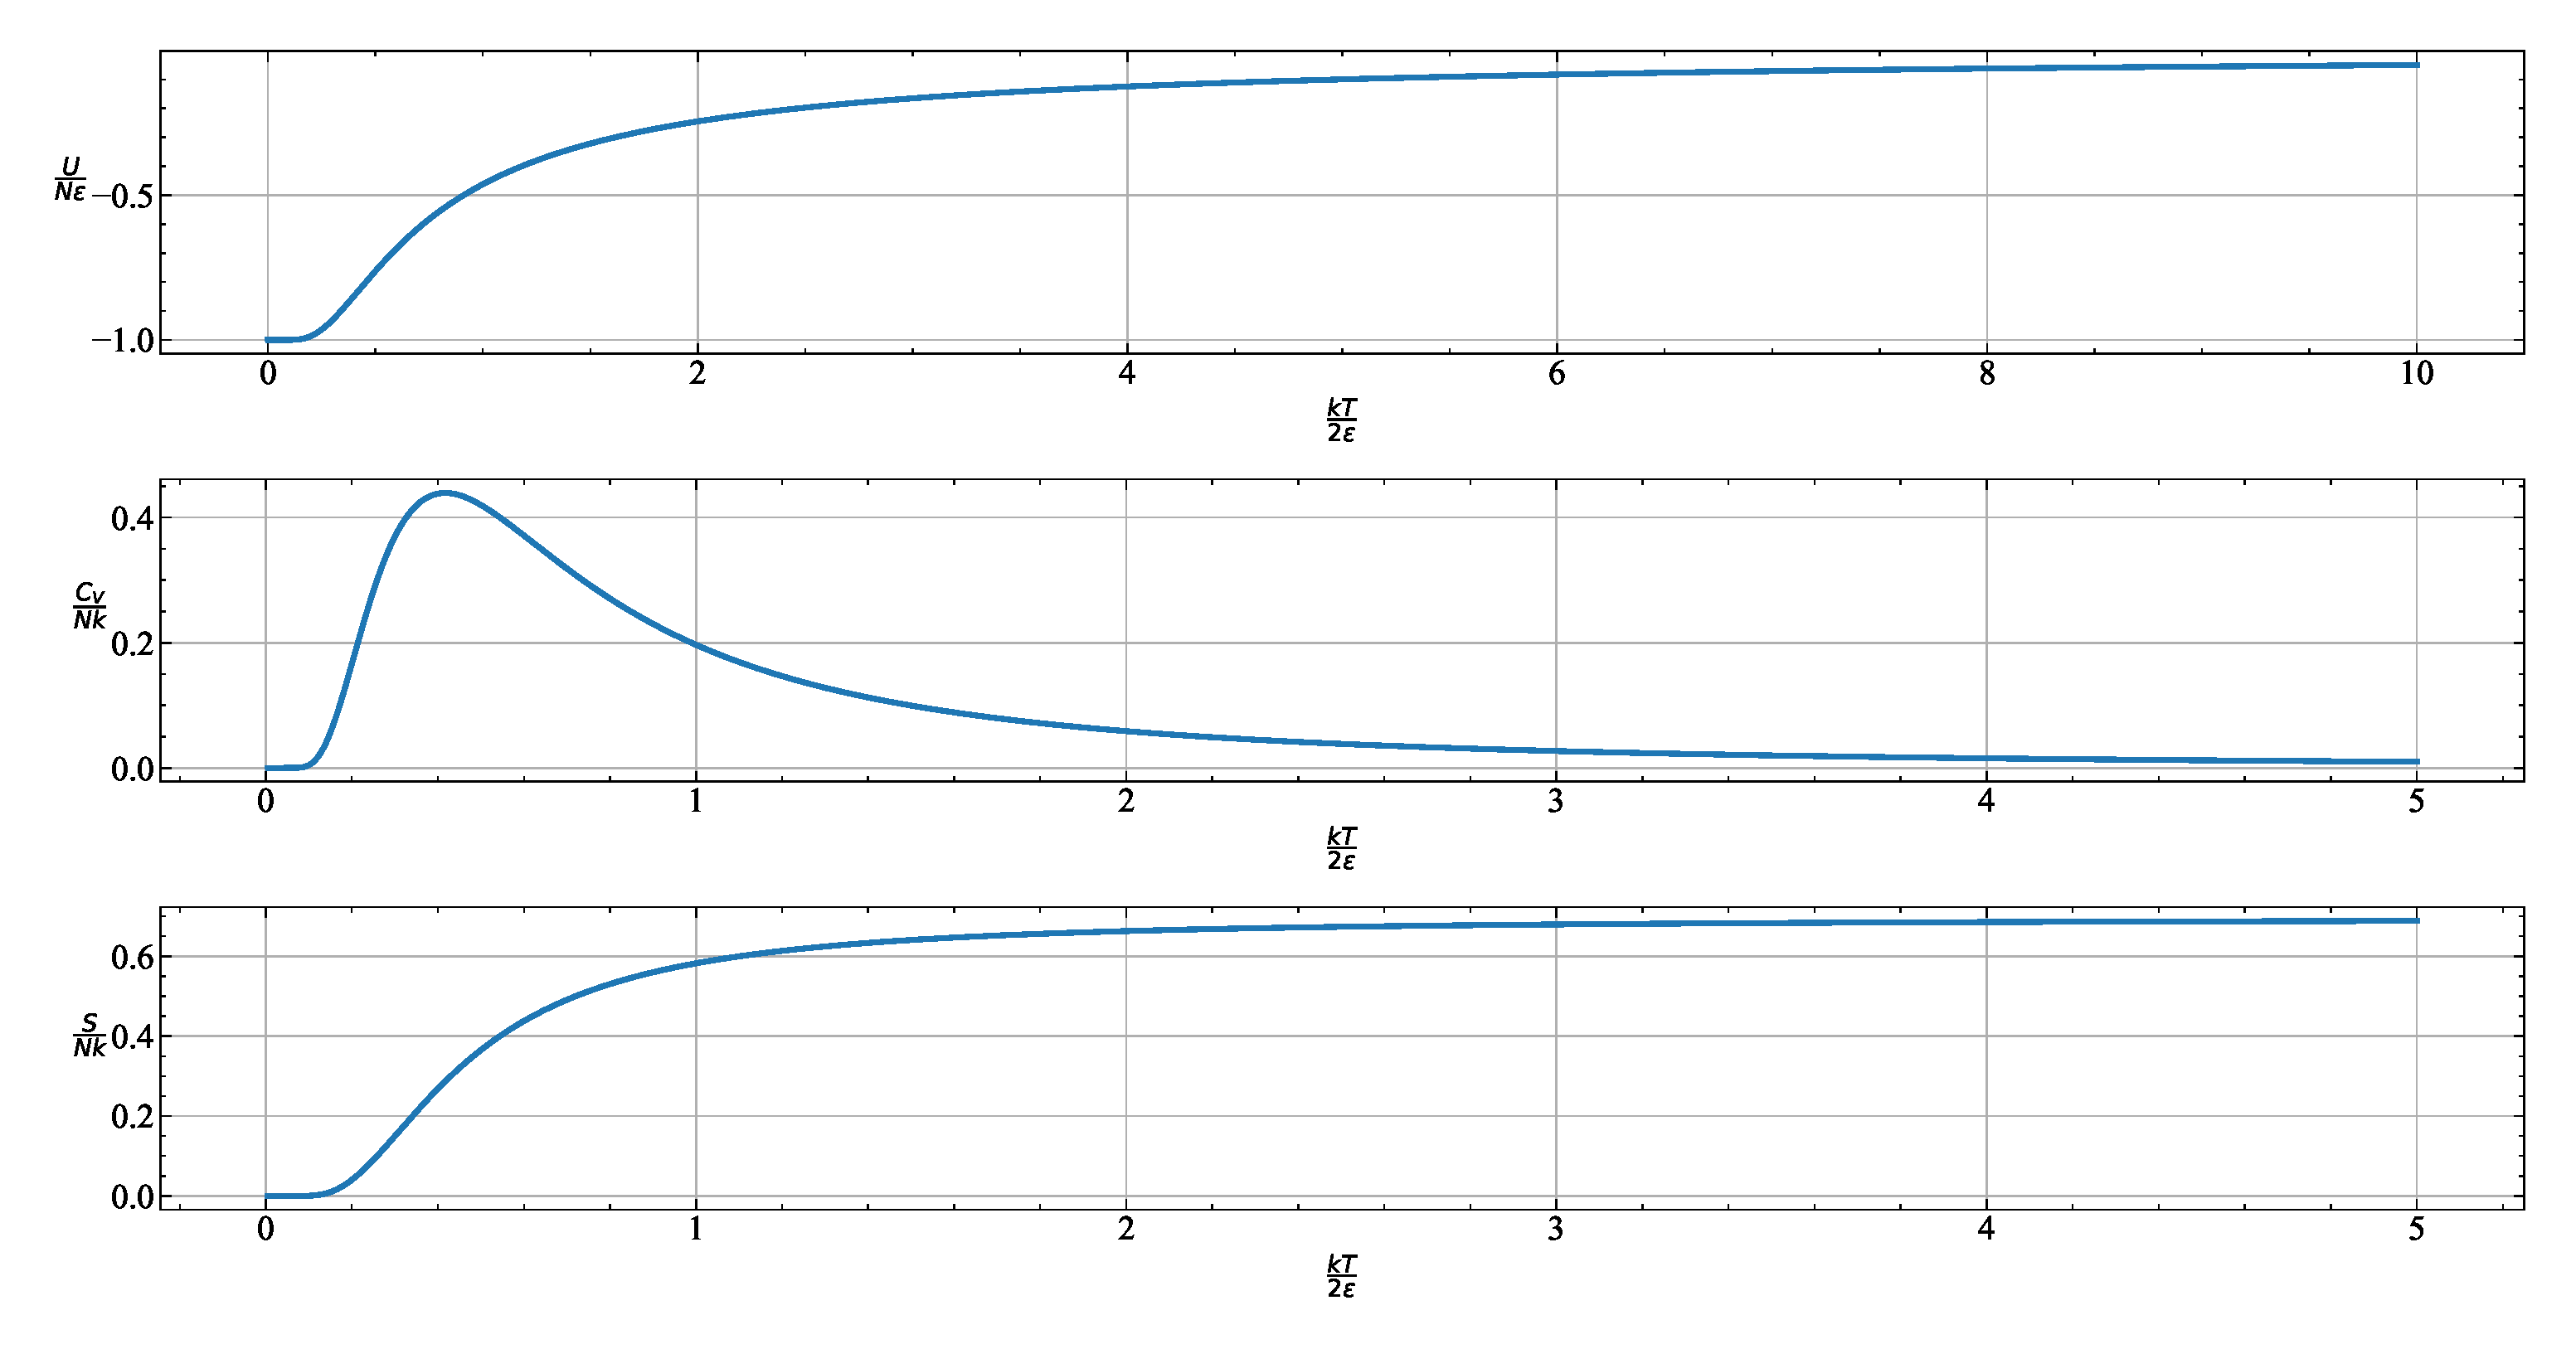
\includegraphics[width=\textwidth]{../../Figure/热统/系综理论/二能级系统热力学量.eps}
    \caption{图中自上而下展示了二能级系统的内能、热容、熵随温度的变化，采用的坐标为归一化坐标。}
\end{figure}
观察热容曲线，明显看出热容随温度呈现先增大后减小的趋势，形成一个峰，被称为肖特基峰。倘若我们测量材料的热容曲线，在某个区域内出现肖特基峰，可能表明材料的基态和第一激发态较近，而别的高能态离它们较远。

最后我们深入分析一下刚刚提到的非平庸的结果。当温度趋于无穷时，我们发现系统的内能并不是趋于\(N\varepsilon\)，也就是说并不是所有粒子都在激发态，而是一半处于基态一半处于激发态。倘若我们让激发态的粒子数再多一点，即使系统的能量大于0，由内能公式我们得到\(T<0\)。从\(\frac{1}{kT}=\left(\pdv{\ln \Omega}{U}\right)_{N,V}\)定性分析，系统能量大于0时，随着激发态粒子变多，系统能量变大，而微观状态数减小，温度作为两者的变化率确实是负的。这是非常诡异的一件事，让一个正能量的系统和负能量的系统热接触，那么正能量的系统要给负能量的系统传递能量，按照热力学的认识，这说明正能量的系统更“热”，也就是\(T<0\)比\(T>0\)更热。定量的分析温度的变化，从\(kT=\frac{2\varepsilon}{\ln(\frac{N}{N_2}-1)}\)可得，在系统变热，也就是\(N_2\)增长的过程中，\(T\)会出现一个无穷间断点，温度先从0变为正无穷，接着间断为负无穷，再增长为0。这告诉我们\(T=0^+\)是最冷的，而\(T=0^-\)是最热的。

听起来这就很不合理。温度不能是负的是热力学的结论，热力学久经考验不大可能是错的。而对于这个二能级系统我们貌似很容易让激发态粒子数超过基态粒子数进而使系统温度为负。问题的产生迫使我们追溯最初的理论假设，回到一切的起点，这说明负温度即系统能量为正是非平衡态\footnote{读者学完热统后可能会有种感触：\(kT\)反应了粒子能量变大的趋势，而系统的稳定总是倾向于能量更小，两种趋势共同作用导致了平衡。如果\(T<0\)，两个趋势都是粒子能量降低，那么系统必然不会是平衡态。当然这是笔者的感触，大家权且一听}。计算二能级系统的热力学量，统计部分的内容我们只用到了玻尔兹曼公式，它对于系统的平衡没有要求，后续我们又用平衡态热力学理论分析，两相矛盾，得出一些奇异的结论也无可厚非。正如我们的二能级系统，要让系统出现负温度这种特列，必要的条件是系统的能量有上限，感兴趣的读者可以自行深入了解。

\section{理想气体}

本节我们处理经典理想气体，即热力学中所说的温度足够高、压强足够小，足够稀薄的气体系统，这样的气体系统是满足非简并条件的。我们假设气体分子是单原子分子，也就是我们只考虑理想气体的平动。假设理想气体分子在一个边长为\(L\)的立方体盒子里，则\(V=L^3\)，分子数为\(N\)，系统的能量为\(E\)。我们先假设气体分子是可分辨的，这本身就是计算的必要步骤，同时我们展示这会得到什么错误结论。

根据微正则系综的理论，我们的首要任务是求出系统在给定约束下的微观状态数。对于二能级系统，这非常简单，但对于理想气体，我们就要花一番力气了。只考虑平动，气体分子可视为三维立方盒子中的自由粒子，其能量为\(E_{n_x,n_y,n_z}=\frac{\hbar^2\pi^2(n_x^2+n_y^2+n_z^2)}{2mL^2}\)。\(N\)个分子的能量和就是系统的能量\(E\)即
\begin{equation}
    \sum_{i=1}^{N} \frac{\hbar^2\pi^2(n_{ix}^2+n_{iy}^2+n_{iz}^2)}{2mL^2}=E \quad n_{ix},n_{iy},n_{iz}=1,2,\dots
\end{equation}
对于玻尔兹曼系统，确定其微观状态就是确定各粒子的量子态。理想气体系统中每个粒子的量子态由3个量子数给定，也就是说确定系统的微观状态要确定\(3N\)的量子数，显然这\(3N\)个量子数就是上述方程的解。那么系统的微观状态数就是上述方程的解的个数。为了计算这个方程的解的个数，我们要先介绍一下“球”的体积公式。
\begin{example}
    求\(n\)维欧几里得空间中半径为\(R\)的球的体积。
    \begin{solution}
        \(n\)维欧几里得空间中半径为\(R\)的球，即空间中到原点距离小于等于\(R\)的点构成的集合。这个概念是三维空间中球的概念的外延，它的体积也是球的体积这一概念的外延，比如2维球的体积其实是圆的面积。用\(V_n(R)\)表示\(n\)维球的体积，显然\(V_2(R)=\pi R^2\)，\(V_3(R)=\frac{4\pi}{3}R^3\)，不难想到\(V_n(R)=A_nR^n\)，其中\(A_n\)是常数。跟\(n\)维球绑定的一个概念是\(n-1\)维\footnote{这里的维度类似自由度，是确定这个几何体所需的坐标数，比如3维球的表面，其显然是2维的}球面，即\(n\)维球的表面。它的大小用面积\(S_{n-1}\)来度量，这是球面面积的外延，比如1维球面的面积其实就是圆的周长。不难得到\(\displaystyle S_{n-1}=\dv{V_n}{R}=nA_nR^{n-1}\)。

        为了计算\(V_n(R)\)，我们采用两种方法计算高斯积分
        \begin{equation*}
            I=\int_{-\infty}^{\infty}\dd x_1\int_{-\infty}^{\infty}\dd x_2\cdots\int_{-\infty}^{\infty}\dd x_n\exp(-\sum_{i=1}^{n}x_i^2)
        \end{equation*}
        这是\(n\)维高斯积分，可以拆成一维高斯积分，即
        \begin{equation*}
            I=\left(\int_{-\infty}^{\infty}\mathrm{e}^{-x^2}\dd x\right)^n=\pi^{\frac{n}{2}}
        \end{equation*}
        另一方面，我们可以采用\(n\)维球坐标计算高斯积分。令\(\displaystyle \sum_{i=1}^{n}x_i^2=r^2\)则
        \begin{equation*}
            I=\int_{\text{全空间}}\mathrm{e}^{-r^2}\dd V
        \end{equation*}
        问题是如何确定\(n\)维球坐标中的体积元\(\dd V\)。注意到被积函数\(\mathrm{e}^{-r^2}\)仅是\(r\)的函数，类比三维空间球坐标，此时的体积元可以表示成
        \begin{equation*}
            \dd V=S_{n-1}\dd r=nA_nr^{n-1}\dd r
        \end{equation*}
        因此高斯积分可表示为
        \begin{equation*}
            I=nA_n\int_{0}^{\infty}r^{n-1}\mathrm{e}^{-r^2}\dd r\xlongequal{r^2=x}\frac{n}{2}A_n\int_{0}^{\infty}x^{\frac{n}{2}-1}\mathrm{e}^{-x}\dd x=\frac{n}{2}A_n\Gamma\left(\frac{n}{2}\right)
        \end{equation*}
        上式最后用到的伽马函数的定义\(\Gamma(n)=\int_{0}^{\infty}x^{n-1}\mathrm{e}^{-x}\dd x\)。两种高斯积分的算法结果显然是一致的，由此可得\footnote{使用伽马函数的递推性质\(\Gamma(n+1)=n\Gamma(n)\)}\(n\)维球的体积为
        \begin{equation}
            V_n(R)=A_nR^n=\frac{\pi^{\frac{n}{2}}}{\frac{n}{2}\Gamma\left(\frac{n}{2}\right)}R^n=\frac{\pi^{\frac{n}{2}}}{\Gamma\left(\frac{n}{2}+1\right)}R^n
        \end{equation}
    \end{solution}
\end{example}

我们把系统的能量约束方程改为
\begin{equation*}
    \sum_{i=1}^{3N}x_i^2=\frac{2mL^2E}{\hbar^2\pi^2} \quad x_i=1,2,\dots
\end{equation*}
显然方程的解位于\(3N\)维空间中的一个球面上，又因为\(x_i\)只能是离散的正整数，因此这个\(3N\)维空间实际上是一个\(3N\)维点阵，方程解的个数就是球面上的格点数。严格计算这个点数是不可能的，因此我们要引入一些物理上的见解。理论上来说，孤立系统的能量也不是一个严格的定值\footnote{真空不空，因此孤立系统不孤立}，实验上来说，能量的测量也总是受到仪器精度的限制，因此我们允许系统的能量有一定的展宽，即\(U-\Delta\leqslant E\leqslant U+\Delta\)，其中\(\Delta\ll U\)可以认为是测量仪器的分辨率。令\(\frac{2mL^2E}{\hbar^2\pi^2}=R^2\)，显然\(R\)也有一定的展宽\footnote{记\(R=k\sqrt{E}\)，则\(R_0=k\sqrt{U}\)，\(\Delta_R=k\sqrt{U+\Delta}-k\sqrt{U}\approx k\frac{\Delta}{2\sqrt{U}}=\frac{R_0}{2}\frac{\Delta}{U}\ll R_0\)}\(\Delta_{R}\ll R_0=\sqrt{\frac{2mL^2U}{\hbar^2\pi^2}}\)。

这样之后，方程的解的个数就变成了\(3N\)维空间中一个薄球壳内的格点数。因为解是正整数，所以格点之间的间距都是1，也就是说平均一个格点的体积为\(1^{3N}=1\)，那么薄球壳内格点的个数就是薄球壳的体积。同样因为解是正整数，所以这里的薄球壳只存在于所有坐标均为正的卦限里，类比三维空间，这部分的体积是整个薄球壳体积的\(\left(\frac{1}{2}\right)^{3N}\)，因此系统的微观状态数可以写成\footnote{此处使用了\(\Gamma(\frac{3N}{2}+1)=(3N/2)!\)，这要求\(N\)为偶数，对于宏观系统，粒子数多一少一没有任何影响，完全可以认为是偶数}
\begin{equation}
    \begin{split}
        \Omega&=\left(\frac{1}{2}\right)^{3N}\bigg[V_{3N}(R_0+\Delta_R)-V_{3N}(R_0-\Delta_R)\bigg] \\
        &=\left(\frac{1}{2}\right)^{3N}\frac{\pi^{3N/2}}{(3N/2)!}R_0^{3N}\left[\left(1+\frac{\Delta_R}{R_0}\right)^{3N}-\left(1-\frac{\Delta_R}{R_0}\right)^{3N}\right] \\
        &\approx \left(\frac{1}{2}\right)^{3N}\frac{\pi^{3N/2}}{(3N/2)!}R_0^{3N}\left(6N\frac{\Delta_R}{R_0}\right) \\
        &=6N\left(\frac{1}{2}\right)^{3N}\frac{\pi^{3N/2}}{(3N/2)!}R_0^{3N-1}\Delta_R
    \end{split}
\end{equation}
我们确实求出来一个微观状态数，但它依赖于能量的展宽，这是我们在理论建模时候引入的，实际上并不知道，这怎么办？很幸运，“取对数”又来帮助我们了，我们计算一下这个薄球壳的体积和半径为\(R_0\)的球的体积比，这等价于系统的微观状态数和系统能量小于等于\(U\)时的微观状态数之比
\begin{equation}
    \begin{split}
        \frac{\Omega}{\Gamma}&=\frac{V_{3N}(R_0+\Delta_R)-V_{3N}(R_0-\Delta_R)}{V_{3N}(R_0)} \\
        &=\frac{(R_0+\Delta_R)^{3N}-(R_0-\Delta_R)^{3N}}{R_0^{3N}} \\
        &=\left(1+\frac{\Delta_R}{R_0}\right)^{3N}-\left(1-\frac{\Delta_R}{R_0}\right)^{3N} \\
        &\approx 6N\frac{\Delta_R}{R_0} \approx 3N\frac{\Delta}{U}
    \end{split}
\end{equation}
\(\frac{\Delta}{U}\)表示系统能量的相对展宽，可以认为是不变的\footnote{物理学中两个量比值远远小于1并不代表比值趋于0，它表示比值是一个足够小的正数以至于泰勒展开式的高阶项可以忽略的。另外后文会看到封闭宏观系统，能量相对涨落约为\(\frac{1}{\sqrt{N}}\)}，对于热力学极限，上式是多项式发散的\footnote{这意味着高维空间中的几何是异常奇怪的，取空间维数为\(10^{24}\)，读者可以计算一下在单位球表面向球内取一个薄球壳，球壳多宽时薄球壳的体积是整个球的体积的\(99.9\%\)。这个球壳占据了球几乎所有的体积但它确实非常薄}。我们已经有了经验，两式之比若是多项式发散，那么它们的对数之比是收敛的，因此我们可以用\(\Gamma\)代替\(\Omega\)计算系统的熵，即
\begin{equation*}
    \frac{S}{k}=\ln\Gamma=\ln\left[\left(\frac{1}{2}\right)^{3N}\frac{\pi^{3N/2}}{(3N/2)!}R_0^{3N}\right]
\end{equation*}

暂时不对这个表达式化简，我们先计算一下理想气体的内能公式
\begin{equation*}
    \frac{1}{kT}=\pdv{\ln\Gamma}{U}=\pdv{\ln\Gamma}{R_0}\pdv{R_0}{U}=3N\frac{1}{R_0}\pdv{R_0}{U}
\end{equation*}
为计算\(\pdv{R_0}{U}\)只需\(R_0^2=\frac{2mL^2U}{\hbar^2\pi^2}\)左右两边同时对\(U\)求导即可
\begin{equation*}
    2R_0\pdv{R_0}{U}=\frac{2mL^2}{\hbar^2\pi^2}=\frac{R_0^2}{U}
\end{equation*}
整理后得到
\begin{equation}
    U=\frac{3}{2}NkT
\end{equation}
接下来计算理想气体的压强即物态方程
\begin{equation*}
    \frac{p}{kT}=\pdv{\ln\Gamma}{V}=3N\frac{1}{R_0}\pdv{R_0}{L}\pdv{L}{V}
\end{equation*}
计算\(\pdv{R_0}{L}\)的思路与上面类似
\begin{equation*}
    2R_0\pdv{R_0}{L}=2\frac{2mLU}{\hbar^2\pi^2}=2\frac{R_0^2}{L}
\end{equation*}
整理后得到
\begin{equation}
    pV=NkT
\end{equation}
这与热力学中的理想气体物态方程意义完全一致，我们借助一个实际的宏观系统印证了统计物理的可行性。与\(pV=nRT\)进行数值上的对比，我们就能得到玻尔兹曼常数在国际单位制下的数值
\begin{equation}
    k=\frac{n}{N}R=\frac{R}{N_A}
\end{equation}
把上述关系带回内能公式可得\(U=\frac{3}{2}nRT\)，这和分子动理论中的能量均分定理是一致的。

现在我们处理熵的表达式
\begin{equation*}
    \begin{split}
        \frac{S}{k}&=\ln\left[\left(\frac{1}{2}\right)^{3N}\frac{\pi^{3N/2}}{(3N/2)!}R_0^{3N}\right] \\
        &=-3N\ln2+\frac{3}{2}N\ln\pi-\ln\frac{3}{2}N!+3N\ln R_0 \\
        &=-3N\ln2+\frac{3}{2}N\ln\pi-\frac{3}{2}N\ln\frac{3}{2}N+\frac{3}{2}N+\frac{3}{2}N\ln(\frac{2mV^{\frac{2}{3}}U}{\hbar^2\pi^2}) \\
        &=\frac{3}{2}N\ln(\frac{1}{4}\pi\frac{2}{3N}\frac{2mV^{\frac{2}{3}}U}{\hbar^2\pi^2})+\frac{3}{2}N \\
        &=\frac{3}{2}N\ln(\frac{mV^{\frac{2}{3}}U}{3N\hbar^2\pi})+\frac{3}{2}N \\
        &=N\ln\left[\frac{V}{\hbar^3}\left(\frac{mU}{3N\pi}\right)^{\frac{2}{3}}\right]+\frac{3}{2}N
    \end{split}
\end{equation*}
把内能公式带入上式可得
\begin{equation}
    S=kN\ln\left[\frac{V}{\hbar^3}\left(\frac{mkT}{2\pi}\right)^{\frac{2}{3}}\right]+\frac{3}{2}kN
\end{equation}
我们把理想气体当成玻尔兹曼系统得到上述熵公式，这肯定是有问题的，问题就在这个熵不具备广延性。简单的验算就发现\(S(2N,2V,T)\neq 2S(N,V,T)\)，这意味着我们用隔板隔开两个完全相同的理想气体，抽取隔板后整个系统会有熵增，这就是所谓的混合熵，但同种理想气体混合是没有混合熵的。另一方面假如隔板两侧的气体\footnote{我们假设两侧气体的粒子数、体积、温度相同，只是粒子属性不同}是异种气体，不难计算出此时的混合熵为\(2nR\ln2\)，这和热力学的结果一致。所以上述熵公式不管是否是同种气体都给出相同的混合熵，是有问题的。

熵来自微观状态数的对数，所以肯定是微观状态数数错了。其实前文已经铺垫良久了，理想气体分子是不可分辨粒子，但满足非简并条件，因此不需要区分其为费米子或玻色子，它的微观状态数由可分辨情形下的微观状态数除以\(N!\)给出，即
\begin{equation}
    \frac{S}{k}=\ln\Gamma-\ln N!
\end{equation}
容易看出修正后的熵公式为
\begin{equation}
    S=kN\ln\left[\frac{V}{N\hbar^3}\left(\frac{mkT}{2\pi}\right)^{\frac{2}{3}}\right]+\frac{5}{2}kN
\end{equation}
显然上述熵是满足广延性的，也容易验算对于异种气体混合给出的混合熵也是\(2nR\ln 2\)。

关于理想气体的统计远没有结束，我们对上述熵公式做一些极限分析。取低温极限，上述熵是发散的，这肯定不对。问题出在哪呢？依旧是微观状态数的问题。经典理想气体足够稀薄才满足非简并条件，对于低温气体，已经不再稀薄\footnote{读者可能困惑，温度不改变粒子数密度为什么会使气体不再稀薄。其实稀薄本身就是相对概念，一定是由粒子数密度和另一个物理量的比较而决定的，后文我们会给出稀薄的明确定义}，自然不满足非简并条件，在这种情况下，我们要抛弃玻尔兹曼系统的舒适区，完全进入不可分辨统计的领域。这种要完整考虑不可分辨性的气体系统称为量子理想气体，是本科统计物理课程的重要研究对象。取高温极限，仅从熵公式来说貌似没什么问题，但我们在计算微观状态数时使用的能级公式是非相对论自由粒子的能级公式，当温度很高粒子能量很大时我们就要考虑相对论效应了。这些极限分析反映的问题也是可以预见的，因为我们统计的对象是经典理想气体，“经典”就意味着它处于非量子非相对论的经典物理领域，当进入量子的、相对论的领域，经典理想气体这个模型本身已不再适用了。


\end{document}
